\ifdefined\IRFAPREPRINT
  \documentclass[preprint,12pt,authoryear]{elsarticle}
\else
  \documentclass[final,5p,times,twocolumn,authoryear]{elsarticle}
\fi
\usepackage{amsmath,amssymb,amsthm,booktabs,graphicx,threeparttable,longtable,array,tabularx,multirow}
\usepackage{xcolor}
\usepackage{stfloats}
\usepackage{flushend}
\usepackage{hyperref}
% Let wide exhibits share pages with text and cross subsection boundaries.
% Keep font sizes and exhibit dimensions unchanged; avoid half-empty float pages.
\setcounter{topnumber}{3}
\setcounter{bottomnumber}{2}
\setcounter{totalnumber}{4}
\setcounter{dbltopnumber}{2}
\renewcommand{\topfraction}{0.88}
\renewcommand{\bottomfraction}{0.72}
\renewcommand{\textfraction}{0.10}
\renewcommand{\floatpagefraction}{0.85}
\renewcommand{\dbltopfraction}{0.88}
\renewcommand{\dblfloatpagefraction}{0.85}
\ifdefined\IRFAREADER
  \usepackage{fancyhdr}
  \fancypagestyle{irfareader}{%
    \fancyhf{}
    \fancyhead[L]{\footnotesize International Review of Financial Analysis}
    \fancyhead[R]{\footnotesize Author manuscript preview}
    \fancyfoot[C]{\footnotesize\thepage}
    \renewcommand{\headrulewidth}{0.4pt}
    \renewcommand{\footrulewidth}{0pt}}
\fi
\hypersetup{colorlinks=true,linkcolor=black,citecolor=black,urlcolor=blue}
\emergencystretch=2em
\journal{International Review of Financial Analysis}
\newtheorem{proposition}{Proposition}
\newtheorem{corollary}{Corollary}
\newcommand{\E}{\mathbb{E}}
\newcommand{\Pp}{\mathbb{P}}
\newcommand{\Loss}{\mathcal{L}}
\newcommand{\Kset}{\mathcal{K}}
\ifdefined\IRFAPREPRINT
  \newenvironment{widefigure}[1][!tbp]{\begin{figure}[#1]}{\end{figure}}
  \newenvironment{widetable}[1][!tbp]{\begin{table}[#1]}{\end{table}}
\else
  \newenvironment{widefigure}[1][!tbp]{\begin{figure*}[#1]}{\end{figure*}}
  \newenvironment{widetable}[1][!tbp]{\begin{table*}[#1]}{\end{table*}}
\fi

\begin{document}
\begin{frontmatter}
\title{Low-Dimensional Asset-Pricing Networks: Identification, Stability, and Economic Use}
\ifdefined\IRFAAUTHORED
\author[aff1]{Jinpeng Wang}
\ead{wangjp@gcu.edu.cn}
\ead[url]{https://orcid.org/0009-0003-7324-2211}
\author[aff1]{Yan Jiang\corref{cor1}}
\ead{jiangyan@gcu.edu.cn}
\ead[url]{https://orcid.org/0009-0004-0250-7486}
\cortext[cor1]{Corresponding author. International Business School, Guangzhou City University of Technology, No. 1 Xuefu Road, Guangzhou 510800, China.}
\affiliation[aff1]{organization={International Business School, Guangzhou City University of Technology},addressline={No. 1 Xuefu Road},city={Guangzhou},postcode={510800},country={China}}

\fi

\begin{abstract}
Low-dimensional representations in asset-pricing networks can summarize data without identifying a unique number of priced directions. We examine this distinction using U.S. equity models, a known-loading simulation, and a separate forecast-updating exercise. Across 30 models per characteristic specification, the selected dimension depends on test assets, loss weighting, random seeds, data construction, and evaluation period. A locked 2020--2025 evaluation supports one of four prespecified directional criteria, with imprecise market-attenuation estimates. Earlier legacy development overlaps January 2020, so this period is not an untouched holdout for the entire research process. In the simulation, noisy evaluation reduces average exact-dimension recovery from 64.2\% to 32.6\%; a finite nested Gaussian example explains persistent over-selection. Hidden-layer median participation rank declines from 20.25 to 9.05, but adding final-layer geometry improves held-out prediction of model-level pricing loss by only 3.915\%, below the specified 5\% threshold. In separate return predictors, retrospective changes in updating value do not yield significant incremental after-cost gains under the tested real-time rule. These results support reporting dimension rankings and uncertainty conditional on the assets, measurement, and evaluation criterion, rather than interpreting a validation minimum as an invariant economic dimension.
\end{abstract}

\begin{keyword}
Machine learning \sep Asset pricing \sep Pricing dimension \sep Model instability \sep Representation geometry \sep Real-time updating
\end{keyword}

\end{frontmatter}
% Keep natural paragraph spacing below tall floats instead of stretching gaps.
\raggedbottom
\ifdefined\IRFAREADER\pagestyle{irfareader}\fi

\noindent\textbf{JEL classification:} G12; C52; C53; C55.

\section{Introduction}

Machine-learning asset-pricing models can use many firm characteristics while producing a small number of latent factors or concentrated hidden representations. This raises an identification question: does a compact fitted representation reveal an economic dimension, or does it summarize the information that matters for a particular sample and evaluation criterion? The distinction matters when a selected network width is interpreted as the number of priced risks or used to fix model complexity over time.

Flexible return predictors and characteristic-based factor models provide several ways to summarize the cross-section \citep{gu2020empirical,kelly2019characteristics,gu2021autoencoder,chen2024deep}. Their statistical and economic objects differ. A low effective rank of activations measures concentration; a small factor set concerns a payoff span; a minimum validation loss identifies a preferred candidate under a specified criterion. None of these quantities is automatically the smallest number of structural shocks. We examine the additional evidence needed to connect them. We do not attribute a common structural claim to all of the cited studies.

Our design separates four questions: whether representations concentrate, whether the smallest pricing-sufficient dimension is identified, whether the conclusion persists across measurements and periods, and whether a historically feasible decision rule produces economic gains. These are distinct tests rather than interchangeable measures of model success. The pricing analysis uses six nominal dimensions, five fixed seeds, two archived characteristic pipelines, and several test-asset families. A known-loading simulation isolates statistical selection error. A separate return-prediction replay tests whether retrospective changes in updating value are usable in real time.

The results show substantial dependence on the evaluation design. In development, the ranking of six dimensions changes across weighting geometries and characteristic pipelines; the average rank correlations between the pipelines are negative. Their comparison is descriptive: it combines construction and coverage differences with a one-month difference in return-window timing. Core-86's locked 2020--2025 evaluation retains only one of four prespecified directional criteria, and its market-attenuation intervals include zero. The networks were unchanged, but legacy development had included January 2020, so this later evaluation is not an entirely untouched holdout for the research process.

The simulation provides a statistical explanation for one possible source of instability. Even with known loadings and covariance, an independent noisy evaluation mean can favor an unnecessary direction. We derive this result for a finite nested Gaussian family when training and evaluation samples grow proportionately. A suitable vanishing penalty restores consistency in that design. The argument illustrates a familiar distinction between predictive accuracy and exact model selection \citep{shao1993cv,yang2007cv}; it is not a general theorem for trained neural networks. In the simulation grid, average exact recovery is 64.2\% under population-mean evaluation and 32.6\% under noisy evaluation.

Representation concentration nevertheless appears throughout the frozen network sample. Median participation rank declines from 20.25 to 9.05 across the three hidden layers. Yet final-layer rank adds little to held-out prediction of model-level pricing loss after nominal factor count is controlled for. The separate temporal exercise also distinguishes retrospective patterns from usable rules: updating becomes more aligned with subsequent errors in parts of the later sample, while the tested detector reacts late and the six primary incremental portfolio comparisons fail multiplicity-adjusted significance tests. These return predictors are independent of the pricing-dimension networks; they provide supporting evidence about updating, not a direct test of time variation in the latent pricing dimension.

The contribution is an empirical comparison of these measurement and decision criteria within one documented research sequence. Test assets and weighting matter for pricing conclusions \citep{hansen1997assessing,lewellen2010skeptical}; factor searches require attention to replication and multiplicity \citep{feng2020taming,hou2020replicating}; model comparisons can change after transaction costs \citep{detzel2023costs}. Our evidence connects these issues to the interpretation of compact neural representations. It supports reporting the range of dimensions compatible with a stated loss tolerance, together with the measurement, chronology, and economic-use limitations of that range. It does not establish that a particular alternative selector or monitoring system performs better.

Section~2 develops the framework and the known-loading result. Section~3 describes data, estimators, chronology, and inference. Section~4 reports dimension sensitivity and the simulation. Sections~5 and~6 examine updating and representation geometry, respectively. Section~7 discusses the scope and limitations of the findings.

\section{Related literature and conceptual framework}

\subsection{Flexible prediction and structural pricing objects}

Machine-learning asset pricing has developed along two related lines. The first uses firm characteristics and flexible interactions to predict individual-stock returns \citep{gu2020empirical,avramov2023machine,leippold2022machine}. The second uses characteristics to estimate time-varying exposures, latent factors, or stochastic discount factors (SDFs) \citep{kelly2019characteristics,gu2021autoencoder,chen2024deep,feng2024deep}. Surveys emphasize that these methods can improve prediction and pricing while accommodating a much larger information set than conventional linear specifications \citep{giglio2022factor,bagnara2024review,karolyi2020new}. Recent work also develops formal significance and model-selection procedures for neural or high-dimensional pricing models \citep{fallahgoul2024significance,feng2026stepwise}.

These results establish the value of flexible functional forms, but they do not make the size of a hidden layer or a fitted bottleneck an economic primitive. A predictor can reduce conditional mean-squared error without spanning an SDF that prices a given asset set. A network with many parameters can generate a concentrated representation, while a compact representation can omit a weakly priced direction. We therefore separate predictive complexity, representation dimension, factor dimension, and pricing dimension, and to evaluate each with an object-specific criterion.

Let $Z_t\in\mathbb{R}^{N_t\times p}$ denote the characteristic panel at date $t$, $h_{K,s}(Z_t)$ a fitted representation with nominal output dimension $K$ and training seed $s$, and $F_{K,s,t+1}$ the resulting factor return or SDF innovation. For test-asset excess returns $R_{t+1}\in\mathbb{R}^{J}$, define pricing moments
\begin{equation}
 g_{K,s}=\E[m_{K,s,t+1}R_{t+1}],
\end{equation}
where $m_{K,s,t+1}$ is the scaled SDF associated with the fitted factors. For a positive semidefinite weighting matrix $W$, the population pricing loss is
\begin{equation}
 \Loss_W(K,s)=g_{K,s}'Wg_{K,s}.
 \label{eq:pricing-loss}
\end{equation}
The empirically sufficient dimension is an argmin of an estimate of Eq.~\eqref{eq:pricing-loss}. It is indexed by $W$, the asset vector $R$, the information set used to construct $h$, the fitting sample, and algorithmic randomness. Without additional restrictions it is not an invariant property of the economy.

\subsection{Latent-factor dimension and weak priced directions}

The econometric literature offers consistent procedures for counting pervasive factors from the eigenvalues of large panels \citep{bai2002factors,onatski2010factors,ahn2013eigenvalue}. Asset-pricing applications, however, attach an additional requirement: a direction must matter for pricing, not merely explain covariance. Characteristic-based factor models and supervised latent-factor methods make this distinction operational \citep{kelly2019characteristics,lettau2020factors}. It becomes especially important when risk prices are weak, when the candidate family is nested, or when additional factors are nearly redundant.

Our question is therefore different from estimating the statistical rank of returns. We ask whether the \emph{smallest pricing-sufficient dimension} can be recovered from feasible out-of-sample losses. Cross-validation is well suited to prediction, but selection of a uniquely minimal model requires stronger separation conditions \citep{shao1993cv,yang2007cv,arlot2010cv}. Proposition~\ref{prop:inconsistency} specializes this point to nested pricing models: when larger models share the same population pricing loss and differ only at a higher stochastic order, the raw validation minimum can continue to overselect with positive probability. The simulation section evaluates the size of that problem under controlled truth.

\subsection{Test assets, weighting geometry, and what is identified}

Classical asset-pricing tests make clear that an SDF is assessed through moment restrictions and that the economic distance from a model depends on the return space and its weighting \citep{hansen1991implications,hansen1997assessing,gibbons1989test,shanken1992beta}. Two-pass inference and specification tests further depend on estimated betas, risk prices, and their sampling error \citep{fama1992cross,jagannathan1996conditional,kan2013pricing}. The choice of test assets is consequential: apparently strong fit can arise when the portfolios have a low-dimensional covariance structure or weak exposure to the disputed direction \citep{lewellen2010skeptical}.

These observations imply that a pricing dimension cannot be reported without its measurement geometry. An equal-weighted loss assigns the same coordinate weight to each sample moment. An HJ-type loss rotates and rescales the moment vector using a return second-moment matrix. The factor sets of \citet{fama1993common} and \citet{fama2015five}, characteristic-sorted portfolios, and individual stocks expose different directions. We therefore cross test dimension choices across asset systems and weighting matrices. Disagreement is not treated as a nuisance robustness failure; it is evidence about which parts of the return space identify the claimed dimension.

\subsection{Factor proliferation, model search, and reproducibility}

The factor-zoo literature shows that searching a large menu requires multiple-testing control, shrinkage, and external replication \citep{harvey2016cross,feng2020taming,hou2020replicating}. Many published predictors weaken after discovery \citep{mclean2016destroy}, a smaller subset carries independent information \citep{green2017characteristics}, and regularization can improve pricing when characteristic portfolios contain weak or redundant signals \citep{kozak2020shrinking}. Formal data-snooping procedures provide benchmarks for judging the best rule selected from many candidates \citep{white2000reality,hansen2005spa,romano2005stepwise}. These studies discipline the search over factors or strategies; our paper applies the same logic to the search over dimensions, seeds, losses, data definitions, and historical windows.

Data construction is part of that search space. Characteristic definitions depend on accounting timing, exchange filters, industry mappings, missing-value rules, and cross-sectional transforms. Missing-data treatment can change both the sample and the learned relation \citep{freyberger2025missing}, while interacting anomalies can make apparently separate signals depend on portfolio construction \citep{muller2025interacting}. We therefore treat the legacy 92-characteristic panel and the lineage-audited 86-characteristic panel as two documented measurements of the information set. The resulting sensitivity is economically informative: a dimension that changes when incompletely traceable features are removed may remain predictive, but it is difficult to interpret as a primitive risk count.

\subsection{Representation geometry and functional relevance}

Deep-network representations often occupy a much smaller region than their ambient width suggests. Effective-rank measures summarize spectral concentration \citep{roy2007rank}; nearest-neighbor and likelihood methods estimate local intrinsic dimension \citep{levina2005mle,facco2017twonn}; and layerwise studies document systematic compression in trained networks \citep{ansuini2019intrinsic}. Neural-collapse results provide an important warning that low-dimensional terminal geometry can be created by the training objective itself \citep{papyan2020collapse}. Curvature estimators address a stronger local geometric object \citep{cao2021curvature}. Our tangent-angle diagnostic is a finite-scale comparison, not an implementation of that paper's Weingarten-map estimator. Our numerical-collapse flag is likewise distinct from classification neural collapse.

Representational-similarity methods address a different issue. SVCCA and related canonical-correlation tools compare learned subspaces \citep{raghu2017svcca,morcos2018cca}, while centered kernel alignment (CKA) is invariant to orthogonal transformations and isotropic scaling \citep{kornblith2019similarity}. These tools reveal concentration and drift, but they do not identify which directions price assets. We test one specific form of functional relevance: whether a geometric statistic adds held-out information about a frozen model-level pricing endpoint after conditioning on nominal factor count. This criterion links the measured activations to pricing performance without treating it as the only possible source of economic relevance.

\subsection{Temporal instability, forecast evaluation, and implementation}

Unknown breaks and multiple structural changes can make a full-sample parameter estimate a mixture of distinct regimes \citep{andrews1993instability,bai1998breaks}. Forecast comparisons must then distinguish unconditional average accuracy from conditional performance and account for nested models \citep{diebold1995accuracy,clark2001nested,giacomini2006conditional}. In unstable environments, adaptive combinations can help, but estimation noise and detection delay can erase their theoretical advantage \citep{elliott2004combinations,giacomini2010unstable,smith2021break}. The poor historical record of many equity-premium predictors illustrates why a retrospective fit is not enough \citep{welch2008equity}.

In a nonlinear model, updating changes thousands of parameters at once. The relevant question is not whether two fits differ but whether the change moves forecasts toward subsequently realized returns. For a frozen prediction $f_{it}$, an updated prediction $u_{it}$, and realized return $y_{it}$, define $e_{it}=y_{it}-f_{it}$ and $d_{it}=u_{it}-f_{it}$. The exact difference in squared errors is
\begin{equation}
 (y_{it}-u_{it})^2-(y_{it}-f_{it})^2=d_{it}^2-2e_{it}d_{it}.
 \label{eq:update-decomp}
\end{equation}
Averaging Eq.~\eqref{eq:update-decomp} gives $A-2B$, where $A=\E[d^2]$ is adjustment cost and $B=\E[ed]$ is alignment with the error of the frozen model. Updating helps only when alignment is large enough to exceed half the adjustment cost. This identity turns the vague idea of model drift into an economically interpretable tradeoff.

Even a favorable prediction result need not be investable. Naive rules can outperform estimated optimal portfolios because parameter uncertainty is costly \citep{demiguel2009optimal}, and turnover and trading costs can reverse model rankings \citep{detzel2023costs}. We therefore distinguish a retrospective change in $A$ and $B$, a detection rule that uses only lagged information, and a portfolio comparison after costs and multiplicity correction.

\subsection{Four claims and their evidence}

Table~\ref{tab:propositions} distinguishes four claims. They are an organizing framework, not a theorem that all four are necessary for every valid economic model. In particular, a pricing model need not generate trading alpha to be economically meaningful. The implementation criterion applies when the claim concerns a usable updating policy.

\begin{widetable}[!tbp]
\centering
\caption{Four claims about low-dimensional pricing representations}
\label{tab:propositions}
\footnotesize
\begin{threeparttable}
\begin{tabularx}{\textwidth}{@{}p{0.12\textwidth}p{0.23\textwidth}X@{}}
\toprule
Claim & Empirical object & Evidence relevant to the stated claim \\
\midrule
Geometry & Rank or local dimension of activations & Decline across layers that survives normalization, estimator checks, and a collapse diagnostic. \\
Exact $K$ & Minimal sufficient $K$ & Recovery under known truth or a valid penalty/equivalence rule; stability cannot be inferred from a single validation minimum. \\
Stability & Invariance of the selected economic object & Agreement across test assets, loss geometries, data definitions, seeds, and nonoverlapping periods. \\
Real time & Economic value of reacting to change & A lag-feasible detection rule and a net portfolio gain after inference, turnover, and transaction costs. \\
\bottomrule
\end{tabularx}
\begin{tablenotes}[flushleft]\footnotesize
\item These criteria concern different objects; success on one criterion does not establish the others.
\end{tablenotes}
\end{threeparttable}
\end{widetable}

Figure~\ref{fig:evidence-ladder} tests the geometry--pricing link directly rather than inferring it from visual concentration. For every frozen network, the open marker is its leave-one-seed-out pricing prediction using nominal factor count alone. The arrow ends at the prediction obtained after adding hidden-layer participation rank. If the compressed representation transported reliably into pricing performance, most arrows would move materially toward the 45-degree line. They do not. Representation concentration and incremental pricing information are evaluated separately.

\begin{widefigure}[!tbp]
\centering
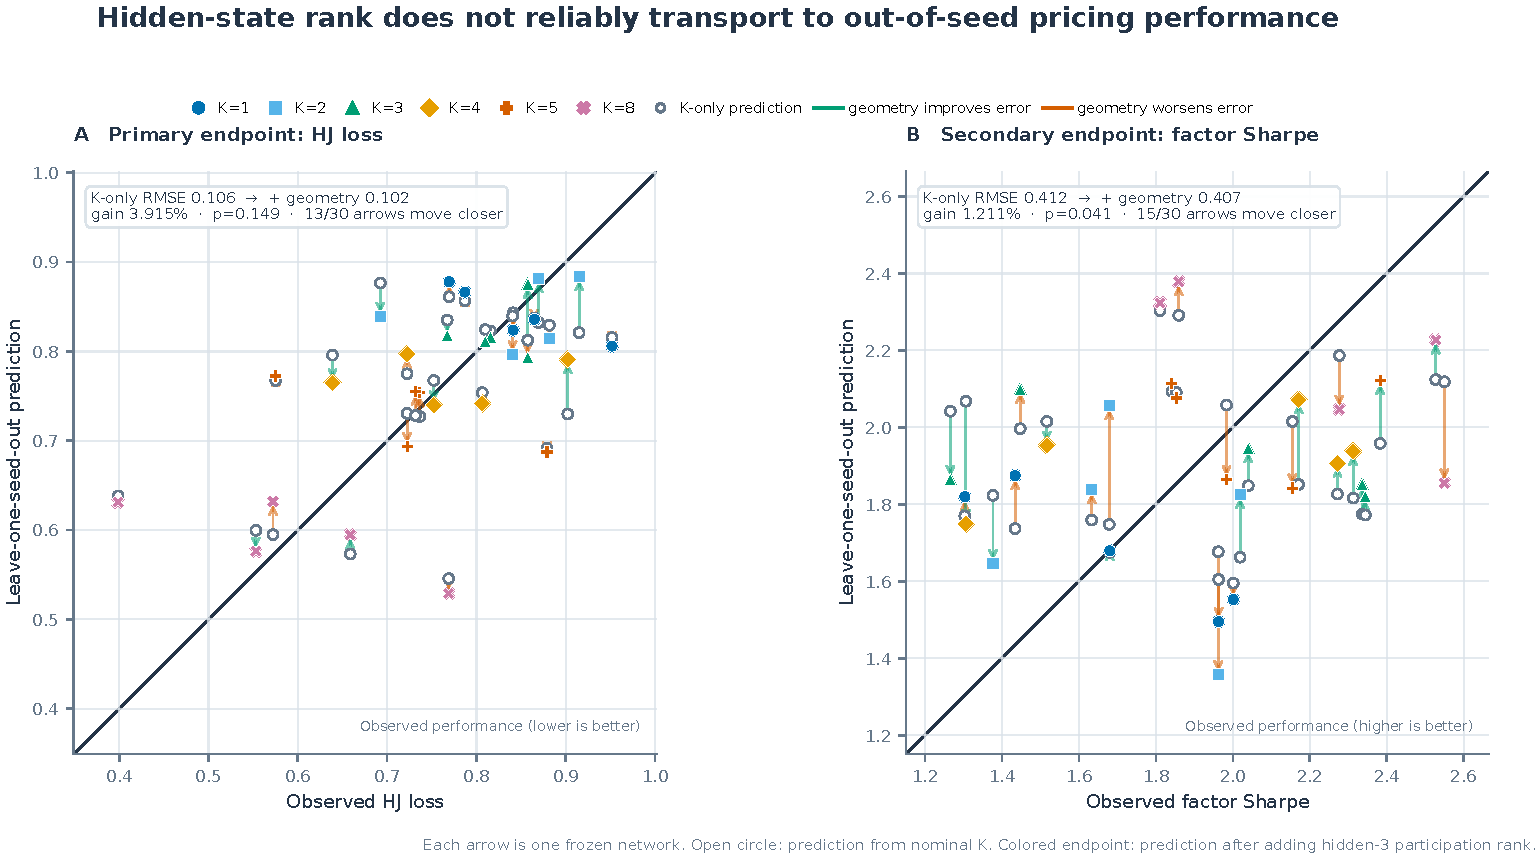
\includegraphics[width=0.98\textwidth]{figures/figure_01_evidence_ladder.pdf}
\caption{Leave-one-seed-out pricing predictions with and without hidden-state geometry. Each arrow is one of 30 frozen networks. Open circles use nominal factor count alone; colored endpoints add hidden-3 raw-centered participation rank, with color and shape identifying nominal $K$. Arrows ending closer to the 45-degree line improve prediction. Geometry reduces HJ-loss RMSE by 3.915\%, below the prespecified 5\% gate ($p=0.149$), and reduces factor-Sharpe RMSE by only 1.211\%. The figure displays the prediction errors behind those aggregate gates rather than rescaled diagnostic ranks.}
\label{fig:evidence-ladder}
\end{widefigure}

\subsection{Why minimum validation loss need not select the minimal dimension}

We give an exact calculation for the known-loading Gaussian design used in Section~4. This is a result about a finite nested family of linear pricing spans, not a consistency theorem for independently trained neural networks.

Let $W$ be fixed and positive definite, and let $P_K$ be the $W$-orthogonal projector onto the span of the first $K$ columns of a full-column-rank loading matrix. The candidate set is finite and contains the smallest correct dimension $K_0$, with $P_{K_0}\mu=\mu$. Independent training and evaluation means satisfy
\begin{equation}
 \bar R_n=\mu+n^{-1/2}U,\qquad
 \bar R_T^{e}=\mu+T^{-1/2}V,
\end{equation}
where $U,V$ are independent $N(0,\Sigma)$ and $\Sigma$ is positive definite. Fit $\widehat\mu_K=P_K\bar R_n$ and evaluate
\begin{equation}
 \widehat\Loss_T(K)=\|\bar R_T^{e}-\widehat\mu_K\|_W^2,
 \qquad \|x\|_W^2=x'Wx.
\end{equation}
For $K>K_0$, put $Q_K=P_K-P_{K_0}$. Orthogonality gives the exact identity
\begin{equation}
 T\{\widehat\Loss_T(K)-\widehat\Loss_T(K_0)\}
 =\frac{T}{n}\|Q_KU\|_W^2
 -2\sqrt{\frac{T}{n}}V'WQ_KU.
 \label{eq:nondegenerate-diff}
\end{equation}

\begin{proposition}[Raw validation selection in the known-loading design]
\label{prop:inconsistency}
Suppose $n/T\to c\in(0,\infty)$ and the candidate set includes at least one $K>K_0$. If every smaller candidate has $\|(I-P_K)\mu\|_W^2>0$, under-selection vanishes but the probability that the unpenalized validation minimizer differs from $K_0$ stays bounded away from zero.
\end{proposition}

Conditional on $U$, the second term in Eq.~\eqref{eq:nondegenerate-diff} is a nondegenerate normal variable whenever $Q_KU\ne0$, an event of probability one. It therefore exceeds the first term with positive probability. An overfitted candidate then beats $K_0$, even as the unscaled loss difference converges to zero. Underfitted candidates instead retain a fixed positive population gap. Supplement~A gives the full argument.

\begin{corollary}[A sufficient penalty rate in this design]
\label{cor:penalty}
For the same finite candidate family, minimizing $\widehat\Loss_T(K)+p_TK$ consistently selects $K_0$ if $p_T\to0$ and $Tp_T\to\infty$.
\end{corollary}

The penalty dominates every $O_p(T^{-1})$ overfit difference while remaining smaller than each fixed underfit gap. With oracle evaluation of the population mean, the cross term in Eq.~\eqref{eq:nondegenerate-diff} is absent and an overfitted candidate cannot improve on $K_0$. Thus the simulation isolates evaluation noise without estimating loadings or the covariance matrix. An estimated weight matrix, different training-to-validation ratio, growing candidate set, or nonlinear fitted family requires a separate analysis. The penalty result is a theoretical benchmark; this paper does not report an empirical comparison of penalty choices.

\section{Data and frozen empirical design}

\subsection{U.S. equity panel and information timing}

The reconstructed stock panel uses CRSP CIZ daily stock data aggregated to calendar months, Compustat North America annual and quarterly records, and CCM link history. It is not a direct extract of the CRSP Monthly Stock File. Monthly returns compound daily total returns after duplicate distribution rows are resolved; the CIZ delisting return is retained rather than added again. The pipeline keeps the frozen common-stock classification and date-valid accounting links. Annual accounts use a six-month lag; quarterly availability uses the recorded reporting date when admissible and a conservative fallback otherwise. These rules limit timing errors but do not turn a current-vintage accounting database into a point-in-time vintage archive.

The reconstructed panel spans 1950--2025. The Core-86 training period contains 437 target-return months from August 1963 through December 1999. Validation and development contain 120 target months each, January 2000--December 2009 and January 2010--December 2019. Characteristic months precede target months by one. The later evaluation contains 72 target months, January 2020--December 2025, and 286,565 stock-month observations.

Core-86 contains 20 monthly/market, 10 quarterly, and 56 annual characteristics. The production input is a documented bridge: it retains nonmissing public benchmark characteristics where available through 2021 and uses audited self-built values otherwise. It is therefore not an entirely independent reconstruction of every historical value. Monthly cross-sectional ranks are mapped to $[-1,1]$; missing ranks are set to zero and accompanied by separate indicators. The 86 characteristics thus generate 172 network inputs. Relative to the earlier 92-characteristic non-announcement benchmark, the omitted columns are \texttt{ms}, \texttt{ps}, \texttt{tb}, \texttt{bm\_ia}, \texttt{chpmia}, and \texttt{pchcapx\_ia}. Supplement~B and the replication package give the variable dictionary and construction scripts.

A chronology limitation affects the legacy comparison. Core-92 used characteristic-month splits: its nominal 2010--2019 development block realizes returns in February 2010--January 2020, whereas Core-86 realizes returns in January 2010--December 2019. Consequently, Core-92/Core-86 differences combine feature membership, reconstruction and coverage, and a one-month shift in the evaluation window. They are a comparison of archived data pipelines, not an isolated six-feature deletion experiment. The overlap also means that January 2020 had entered legacy development before the later 2020--2025 evaluation was fixed. We call that exercise a \emph{locked later-period evaluation}, not a wholly untouched holdout for the research process. Its Core-86 weights and decision rules were fixed before that evaluation.

The analysis avoids corporate announcements, news text, analyst narratives, and language-model embeddings. The information set consists of market and accounting variables whose timing can be encoded as reproducible tabular data. This restriction isolates whether nonlinear pricing structure can be learned from conventional numerical information.

\subsection{Later same-panel feature control}

To isolate feature removal from the archived pipeline contrast, a later paired experiment starts from one Core-92 mother panel. It contains 2,068,593 training, 606,278 validation, and 444,538 development stock-months under the target-month calendar used by Core-86. Both arms load the same ordered rows, ranked values, missingness indicators, returns, and test-asset outcomes. All 184 input positions and hidden widths are retained. In the masked arm only, the six excluded characteristic columns and their six missingness indicators are set to zero. Each of the six $K$ values and five seeds receives the same initial parameter tensors in both arms; optimizer settings and the validation stopping rule are unchanged. This produces 30 pairs, or 60 additional models, without architecture or hyperparameter search.

The primary comparisons are all six fixed-$K$ paired pricing-distance differences for the combined 74 assets at geometry endpoints zero and one. Full curves for all three primary asset families, complete rankings, and winner margins are retained. A thousand common twelve-month circular-block draws resample development months and paired seed clusters while retaining every candidate. Validation SDF coefficients remain fixed; the evaluation return second moment and all losses are recomputed in each draw. Intervals are pointwise, conditional on trained models and validation estimates, and do not establish simultaneous coverage or a unique true $K$.

This experiment was designed after the original findings and initial replication release. Its specification was fixed before it ran, but the historical sample was already familiar. It is a post-study control, not fresh confirmation. It isolates information removal within the chosen panel and training procedure; it does not identify the contribution of coverage, accounting vintage, reconstruction, or timing to every historical pipeline difference.

\subsection{Frozen neural model family}

The main family contains 30 neural pricing models. Nominal factor dimension is
\[
 K\in\{1,2,3,4,5,8\},
\]
and each dimension is estimated under five fixed random seeds, 20260924 through 20260928. All models within a data-definition exercise share the architecture, optimization rule, stopping rule, sample splits, and target construction. Dimension and seed are the planned sources of variation. Model selection uses the validation decade. The development decade and the locked period never alter weights or hyperparameters.

Each network has hidden widths 128, 64, and 32, SiLU activations, and a $K$-wide tanh output. Within a month, output scores are centered and normalized separately to unit gross exposure, producing zero-net-investment characteristic-managed factors. Training minimizes three times normalized ridge-HJ span loss minus 0.25 times the annualized factor-span Sharpe, plus 0.05 times squared off-diagonal factor correlations and 0.001 times portfolio concentration. Only the 25 size--book-to-market assets enter this training loss. AdamW uses learning rate $3\times10^{-4}$, weight decay $10^{-5}$, batches of 120 months, at most 80 epochs, and patience 12. Supplement~B specifies normalization and checkpoint selection.

This family was retained for diagnostics after earlier benchmark-advancement criteria failed. It should not be interpreted as a demonstrated state-of-the-art pricing model. Architecture is constant across $K$ apart from output width, but separately trained networks are not algebraically nested. The known-loading simulation removes optimization and separates this limitation from the statistical selection issue.

Random seeds are algorithmic repetitions. We summarize across them because a claimed economic dimension should not depend on one initialization, but we do not treat five seeds as five independent economic time series. Time-series uncertainty is obtained from the monthly sequence and the prespecified block bootstrap.

\subsection{Test assets and external transport}

The primary test assets are 25 size--book-to-market portfolios, 49 industry portfolios, and their 74-asset union. The two component sets emphasize different economic spans: characteristic-sorted portfolios organize the cross-section by size and valuation, while industries load on sector-specific cash-flow risks. The union is the main broad pricing panel.

Six external families test transport beyond the primary assets: 25 portfolios sorted on size and operating profitability, investment, momentum, accruals, market beta, and residual variance. These assets were fixed before the corresponding development and locked evaluations. They are useful because a direction that is weakly represented in size--value or industry portfolios can be more visible in an economically targeted family.

The locked exercise evaluates all nine sets: the three primary sets and six external sets. It does not add assets after observing 2020--2025 outcomes. Public portfolio returns and factor series can be independently obtained from the Kenneth French Data Library; stock-level model construction requires licensed CRSP and Compustat access.

\subsection{Pricing losses and the geometry path}

For each model, factor self-pricing coefficients are estimated in the validation block and then held fixed. Let $F$ be its validation factor matrix. The coefficient is $b=(F'F/T_v+\eta I)^{-1}\bar F$, with $\eta=10^{-6}\operatorname{tr}(F'F/T_v)/K$ and a numerical floor. Evaluation moments are $\hat g=T_e^{-1}\sum_t(1-b'F_t)R_t$. Alphas are intercepts from evaluation-period time-series regressions, a separate descriptive estimand.

Write the evaluation return second moment as $S=V\operatorname{diag}(\lambda_j)V'$. For $\gamma\in\{0,0.05,\ldots,1\}$, the actual geometry path is
\begin{align}
 d_j(\gamma)&=(\lambda_j+\epsilon)^{-\gamma},\\
 W_\gamma&=\frac{J\,V\operatorname{diag}(d_j(\gamma))V'}{\sum_jd_j(\gamma)\lambda_j},\\
 D_{K,s,A}(\gamma)&=\sqrt{12\hat g'W_\gamma\hat g},
\end{align}
where $\epsilon=10^{-4}\operatorname{tr}(S)/J$. This is a spectral-power path with $\operatorname{tr}(W_\gamma S)=J$, not a linear mixture of endpoint matrices. At zero it is a scaled equal-moment norm; at one it is a scaled regularized HJ-type norm. The displayed values are dimensionless annualized distances, not percentage returns. The evaluation second moment determines the metric; it is not an investor's ex-ante estimate of $W$. Coefficients $b$ remain fixed along the path.

The aggregate best dimension minimizes the seed-mean distance at each $\gamma$. We report the entire six-dimension ordering and seed-level winners in addition to the aggregate optimum. This matters because a common average winner can mask dispersion across training runs.

The market-direction diagnostic estimates each test asset's market beta in the validation decade, freezes that beta, and subtracts the associated market payoff in the development or locked period. Define $A_A=[\bar D_{1,A}(0)-\bar D_{5,A}(0)]-[\bar D_{1,A}(1)-\bar D_{5,A}(1)]$, where bars average the five seeds. Market attenuation is
\begin{equation}
 \Delta_A^{mkt}=|A_A|-|A_A^{hedged}|.
\end{equation}
A positive value means that removing the validation-estimated market direction makes the geometry contrast smaller. Betas are never re-estimated on the evaluation period.

The economic-completion diagnostic augments the one-factor neural representation with the observed market excess return. It evaluates both raw Euler moments and time-series alpha. Joint improvement is required because fitting a dominant unconditional moment can leave relative cross-sectional pricing errors unchanged.

\subsection{Development evidence and locked confirmation}

The development analysis maps the full geometry surface, compares Core-92 and Core-86, evaluates the six external families, decomposes spectral directions, and records the market-hedge diagnostics. It is discovery evidence: the sample informed the final hypotheses even though each underlying run used a frozen local protocol.

The later-period protocol was fixed after the development diagnostics. The January 2020 overlap described above prevents a claim of wholly untouched confirmation. The 30 Core-86 checkpoints were unchanged. Four hypotheses were fixed:
\begin{enumerate}
 \item the best dimension changes across endpoint geometries for the combined assets and for at least four of six external families;
 \item removing the frozen market-beta direction attenuates geometry sensitivity for the combined assets and at least four external families;
 \item adding the market factor to $K=1$ jointly improves raw moments and alpha for at least four external families; and
 \item external families select at least three distinct best dimensions across the endpoints.
\end{enumerate}
The run uses 500 twelve-month circular block-bootstrap draws. Point-estimate gates and confidence intervals are both reported; passing a directional point-estimate rule does not convert an interval that crosses zero into precise evidence.

\subsection{Known-truth identification simulation}

The simulation asks whether the observed instability can arise even when the true dimension is known and neural optimization is absent. It contains 500 Monte Carlo replications for each of 144 base conditions. The design crosses true dimensions $K_0\in\{1,3,5\}$, sample lengths $T\in\{72,240,600\}$, strong and weak risk prices, full and weak-tail asset spanning, factor correlation $\rho\in\{0,0.7\}$, and 25 versus 74 test assets. Six independently drawn asset families and two pricing geometries are evaluated.

The candidate dimensions contain the truth. Both modes estimate risk prices from a noisy training mean. Oracle evaluation compares the fitted mean with the population mean; feasible evaluation compares it with an independent noisy mean of the same sample length. Both modes know the loading matrix and population covariance; ``feasible'' here refers only to evaluation-mean noise. The HJ-labelled simulation weight uses a regularized covariance, whereas the empirical path uses return second moments. This is a mechanism experiment, not a literal replication of the empirical estimator. Because true loadings are provided, any difference between oracle and feasible recovery is attributable to dimension identification and evaluation noise rather than a network failing to optimize.

The simulation was frozen before execution. It generated 576 condition summaries, 3,456 selection-frequency rows, and 864 cross-asset disagreement summaries. A second run using the same code and seeds reproduced all four output files byte for byte. Eight directional mechanism tests were fixed in advance: improvements with sample length, strong prices, and complete spanning; greater under-selection under weak prices; greater cross-asset disagreement with weak-tail spanning; disagreement across geometries; amplification of that disagreement with correlation or weak spanning; and better recovery under oracle evaluation.

\subsection{Scope of the separate temporal replay}

Supplement~D documents a retrospective return-prediction replay with neural, Ridge, and shallow-tree estimators. It is not a refit of the 30 pricing-dimension networks. The stock universe and historical model choices are selected using overlapping research history. Its results are retained as a boundary case for economic-use claims, not a prospective investability test or evidence that latent pricing dimension changes. Section~5 gives the limited conclusion; the numerical results and full implementation remain in the supplement.

\subsection{Hidden-representation geometry}

The geometry sample contains the same 30 frozen Core-86 networks, 120 development months, 384 securities per month, 172 inputs (86 ranked characteristics and 86 missingness indicators), and three hidden layers. For every model, month, and layer we calculate participation rank, entropy rank, PCA90 and PCA95 dimension, and a collapse indicator. Neighbor-based TWO-NN and Levina--Bickel ($k=20$) dimensions and a tangent-angle diagnostic are computed only every twelfth development month (ten months) under raw centering and feature z-scoring. They are not computed under row normalization. We repeat the spectral statistics under raw centering, feature z-scoring, and row-$L_2$ normalization.

Because layer widths differ, we additionally report participation rank divided by width and the later architecture-matched random-network control in Section~6. Its protocol was fixed before that control ran, after the earlier results had been inspected. It does not create an independent confirmation sample.

CKA measures adjacent-layer similarity. Rank-five principal-subspace Grassmann distance measures month-to-month drift. The primary functional probe asks whether hidden geometry improves leave-one-seed-out prediction of development-period HJ loss after controlling for nominal factor count. Advancement requires at least a 5\% RMSE reduction and a within-factor-count permutation $p\leq0.05$. The factor-Sharpe probe is secondary and cannot replace the primary endpoint.

\subsection{Evidence hierarchy and reproducibility}

We label evidence as descriptive, development, exploratory, or locked. ``Prespecified'' denotes a time-stamped local protocol fixed before its run, not registration in an external registry. The label determines permissible interpretation. Development findings motivate hypotheses. A locked failure remains a failure even when a related point estimate has the expected sign. Exploratory break dates cannot be presented as real-time rules. Secondary endpoints cannot rescue failed primary gates.

The project archives protocols, source hashes, model hashes, random seeds, manifests, execution receipts, and derived tables. Licensed raw CRSP and Compustat records cannot be redistributed, but the data dictionary, construction code, source links, and checksums document how licensed researchers can reconstruct the stock-level panel. Exact historical bytes require the same source vintages; current downloads can differ because of vendor revisions. All figures in this manuscript are produced from frozen CSV or JSON outputs; no value is transcribed from an unfrozen interactive analysis.

\section{Pricing dimension: empirical sensitivity and statistical identification}

\subsection{Development-period dimension surfaces}

The preferred dimension changes with the data definition and pricing geometry (Figure~\ref{fig:dev-surfaces}). Each row is a candidate dimension within one feature-lineage--test-asset environment, and each column is one of the 21 evaluation geometries. Cell color measures the percentage pricing-distance loss relative to the pointwise best candidate, so the figure preserves both the winner and the economic size of every model's shortfall. The outlined path follows the winner based on the five-seed mean, while circle size records how many individual seeds select that row. A single model does not dominate every asset family and every geometry. For Core-86, the aggregate endpoint winner for the combined 74 assets moves from $K=2$ under the equal-moment endpoint to $K=4$ under the HJ endpoint. The industry and size--book-to-market sets move from $K=2$ to $K=1$. For Core-92, the equal-moment endpoint selects $K=5$ for all three primary sets, while the HJ endpoint selects $K=1$, $4$, and $8$ for the combined, industry, and size--book-to-market assets.

\begin{widefigure}[!tbp]
\centering
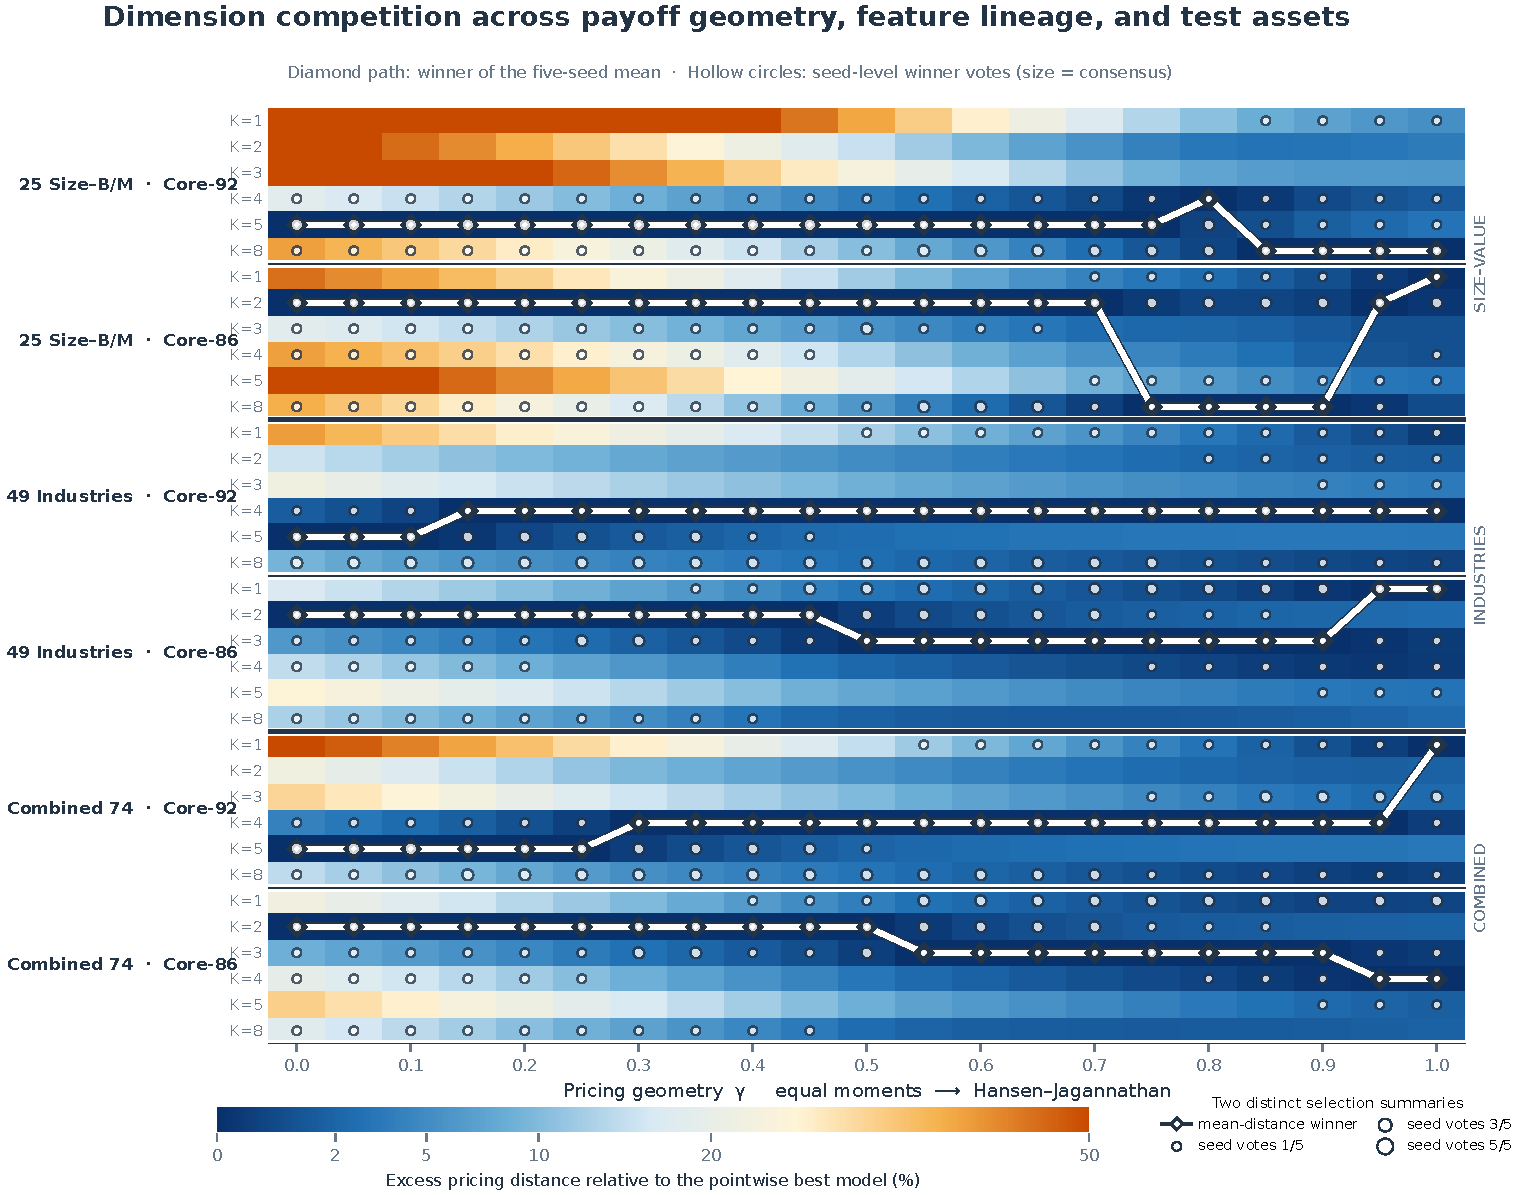
\includegraphics[width=0.98\textwidth]{figures/figure_02_dimension_sensitivity.pdf}
\caption{Empirical dimension-competition field. The 756 cells report every frozen five-seed mean for the archived development windows: two characteristic definitions, three primary test-asset sets, six candidate dimensions, and 21 evaluation geometries. Color is excess pricing distance relative to the best candidate in the same environment and geometry, clipped at 50\% for display; dark blue denotes close competition and orange denotes economically large shortfall. The outlined diamond path follows the winner of the five-seed mean. Hollow circles are a distinct statistic: their area records one to five seed-level winner votes for the corresponding dimension, computed from all 3,780 seed-specific distances. A circle away from the diamond path therefore indicates seed-level support that does not win after averaging. Geometry zero is the equal-moment endpoint and one is the HJ-type endpoint. Core-92 evaluates February 2010--January 2020 returns; Core-86 evaluates January 2010--December 2019 returns. The comparison also changes construction and coverage, not only feature count.}
\label{fig:dev-surfaces}
\end{widefigure}

Table~\ref{tab:dimension-evidence} reports all six candidate dimensions at both endpoints. Its common column structure allows a direct comparison of Core-92 and Core-86 within each asset set. Boldface identifies the seed-mean minimum; neighboring entries show whether that minimum is separated from the alternatives. Parentheses summarize dispersion across five fixed training seeds, not time-series sampling uncertainty.

\begin{widetable}[!tbp]
\centering
\begin{minipage}{\textwidth}
\caption{Pricing distances for every candidate dimension, archived development windows}
\label{tab:dimension-evidence}
\footnotesize
\setlength{\tabcolsep}{4pt}
\renewcommand{\arraystretch}{1.16}
\begin{tabular*}{\linewidth}{@{\extracolsep{\fill}}crrrr@{}}
\toprule
 & \multicolumn{2}{c}{Core-92} & \multicolumn{2}{c}{Core-86} \\
\cmidrule(lr){2-3}\cmidrule(l){4-5}
$K$ & Equal moments & HJ & Equal moments & HJ \\
\midrule
\multicolumn{5}{@{}l}{\textit{A. 25 size--book-to-market portfolios}} \\[2pt]
$1$ & 3.321 (0.183) & 1.840 (0.022) & 2.365 (0.105) & \textbf{1.841} (0.038) \\
$2$ & 2.455 (0.219) & 1.809 (0.036) & \textbf{1.633} (0.143) & 1.843 (0.037) \\
$3$ & 2.725 (0.306) & 1.856 (0.070) & 1.935 (0.167) & 1.858 (0.024) \\
$4$ & 1.893 (0.205) & 1.771 (0.050) & 2.269 (0.391) & 1.857 (0.024) \\
$5$ & \textbf{1.597} (0.314) & 1.798 (0.041) & 2.564 (0.315) & 1.895 (0.054) \\
$8$ & 2.221 (0.336) & \textbf{1.746} (0.047) & 2.236 (0.325) & 1.854 (0.023) \\
\addlinespace[5pt]
\multicolumn{5}{@{}l}{\textit{B. 49 industry portfolios}} \\[2pt]
$1$ & 4.305 (0.126) & 2.332 (0.030) & 3.465 (0.137) & \textbf{2.306} (0.054) \\
$2$ & 3.566 (0.201) & 2.363 (0.048) & \textbf{2.964} (0.130) & 2.365 (0.042) \\
$3$ & 3.771 (0.326) & 2.411 (0.080) & 3.151 (0.117) & 2.311 (0.061) \\
$4$ & 3.137 (0.217) & \textbf{2.328} (0.041) & 3.394 (0.276) & 2.310 (0.044) \\
$5$ & \textbf{3.088} (0.207) & 2.403 (0.041) & 3.718 (0.251) & 2.376 (0.084) \\
$8$ & 3.371 (0.285) & 2.337 (0.041) & 3.348 (0.212) & 2.360 (0.061) \\
\addlinespace[5pt]
\multicolumn{5}{@{}l}{\textit{C. Combined 74 portfolios}} \\[2pt]
$1$ & 5.410 (0.199) & \textbf{2.802} (0.025) & 4.208 (0.168) & 2.750 (0.041) \\
$2$ & 4.343 (0.277) & 2.854 (0.042) & \textbf{3.438} (0.177) & 2.790 (0.033) \\
$3$ & 4.651 (0.433) & 2.867 (0.073) & 3.735 (0.177) & 2.743 (0.055) \\
$4$ & 3.706 (0.277) & 2.808 (0.034) & 4.115 (0.421) & \textbf{2.738} (0.032) \\
$5$ & \textbf{3.559} (0.308) & 2.895 (0.033) & 4.535 (0.362) & 2.785 (0.069) \\
$8$ & 4.067 (0.403) & 2.811 (0.035) & 4.058 (0.324) & 2.788 (0.049) \\
\bottomrule
\end{tabular*}
\par\vspace{4pt}
{\footnotesize\raggedright\textit{Notes:} Each entry is a mean pricing distance over five fixed training seeds; parentheses give the standard error across seeds. Lower is better. Boldface marks the smallest mean within each asset set, data definition, and loss geometry. Seed standard errors describe algorithmic dispersion, not time-series sampling uncertainty. Core-92 return months are February 2010--January 2020; Core-86 return months are January 2010--December 2019. Construction and coverage also differ. All six candidates are shown, including those that never win.\par}
\end{minipage}
\end{widetable}


The result is not merely that two losses produce two answers. The economic content of a pricing error depends on direction. Equal weighting emphasizes the coordinate representation of the moments. HJ weighting discounts directions with large payoff second moments and emphasizes directions that are expensive to span. If weak priced directions are correlated with dominant common directions, a change in $W$ changes the signal-to-noise tradeoff. A dimension claim that is robust only to one geometry is therefore a statement about that loss, not a loss-free risk count.

\subsection{Data-definition and seed instability}

The paired Core-92 and Core-86 row blocks in Figure~\ref{fig:dev-surfaces}, together with Table~\ref{tab:dimension-evidence}, compare the entire six-dimension ordering under the two feature lineages. Exact agreement is nearly absent. Across 21 geometries, the best $K$ agrees twice for the 25 size--book-to-market portfolios, never for industries, and once for the combined assets. Mean Spearman correlations are $-0.355$, $-0.156$, and $-0.151$, respectively; their minima are $-0.600$, $-0.371$, and $-0.371$. Mean Kendall correlations are $-0.263$, $-0.111$, and $-0.124$. The color field also shows that the result is not uniformly driven by economically negligible ties: some switches occur within a broad blue region of near-equivalent models, while others coincide with large orange shortfalls for the displaced candidate. Thus the change reaches beyond a close tie at the minimum; it reverses much of the ordering.

The finding has two interpretations, and the evidence supports only the more cautious one. It could mean that the six excluded signals contain essential pricing information. It could also mean that small changes in measurement, coverage, or missingness shift a weakly identified validation ranking. Because panel definitions are not randomized, we do not assign a causal effect to any excluded variable. Either interpretation weakens the claim that the raw best $K$ is a stable primitive.

Seed sensitivity points in the same direction. There are 12 combinations of data definition, primary asset set, and endpoint geometry. None yields a five-of-five unanimous best dimension. Averaging across seeds is a useful performance summary, but it does not make the underlying structural object seed-invariant. The distinction is analogous to model averaging: aggregation can stabilize a prediction while leaving model selection uncertain.

\subsection{External assets and the common market direction}

In the development period, Core-86 changes best dimension between geometry endpoints for all six external families, but its raw contrast statistic $A$ has a bootstrap interval containing zero in every family. The market-direction attenuation point estimate is positive for five of six families, yet all six intervals contain zero. Adding the market factor to $K=1$ improves raw Euler moments with intervals excluding zero in five of six families, while alpha improvement excludes zero in none. Under Core-92, the same diagnostics appear much stronger: $A$, raw-moment completion, and alpha completion exclude zero for all six families. This difference shows sensitivity between the archived pipelines, which also differ in coverage and timing; it cannot be attributed to data construction alone.

The spectral decomposition provides a coherent economic clue. Compression loss is concentrated in a small number of high-variance common directions. The largest spectral direction is close to the equal-weighted payoff direction, and hedging assets by validation-period market betas reduces the point-estimate geometry contrast. A compact representation can therefore recover aggregate market variation while losing finer relative-pricing information. Adding the market factor can repair a dominant unconditional Euler direction without repairing the cross-section of alphas.

That distinction answers why the direction of compression matters. The decomposition localizes part of the observed error contrast to common payoff variation. It does not establish which information is lost first inside the network, nor identify a causal effect of compression. The absence of joint alpha improvement limits the interpretation to the reported diagnostics.

\subsection{The locked 2020--2025 test}

The development-period dimension pattern does not persist in the locked period (Figure~\ref{fig:sealed-dashboard}). Reading across a row connects endpoint dimension, the raw geometry contrast, market-direction attenuation, raw-moment completion, and alpha completion; hollow diamonds and arrows add the development estimate wherever the same external family is available. Seven of nine asset sets select $K=1$ at both endpoints. Size--accruals and size--residual-variance select $K=1$ under equal moments and $K=8$ under HJ. Combined 74 selects $K=1$ under both. This is a much more uniformly low-dimensional period than development.

\begin{widefigure}[!tbp]
\centering
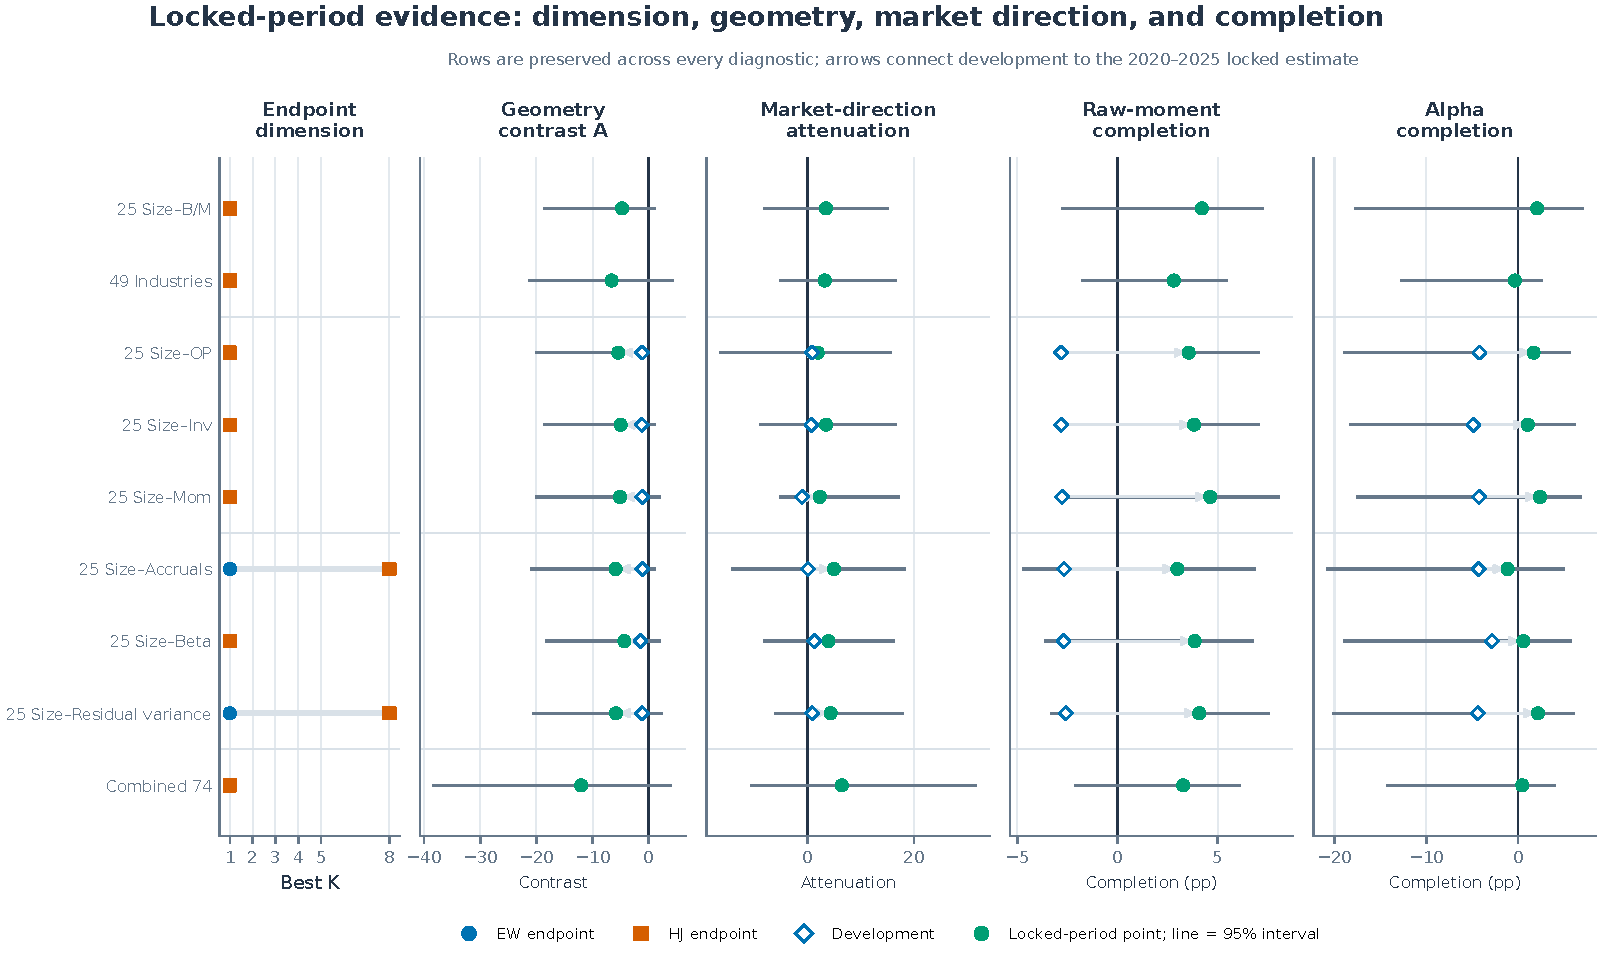
\includegraphics[width=0.99\textwidth]{figures/figure_04_sealed_falsification.pdf}
\caption{Asset-aligned locked 2020--2025 evidence field. Each row preserves one test-asset family across endpoint dimension, raw geometry contrast $A$, market-direction attenuation, raw-moment completion, and alpha completion. Green points and horizontal lines report the locked estimate and its 95\% circular-block interval. For the six external families, hollow diamonds mark the development estimate and arrows point to the locked estimate. The first track compares equal-moment and HJ endpoint dimensions. The Core-86 models and rules were fixed before this later evaluation. Earlier legacy development includes January 2020; the period is not a wholly untouched research holdout.}
\label{fig:sealed-dashboard}
\end{widefigure}

Table~\ref{tab:sealed-evidence} places each asset family's selected dimensions beside its pricing diagnostics and 95\% intervals. The locked evidence supports a directional market effect but does not confirm the broad dimension mechanism. The four frozen decisions follow directly from these rows. Geometry dependence fails because only two of six external families change endpoint dimension, below the four-family threshold, and Combined 74 does not change. The market-direction gate passes its point-estimate rule: attenuation is positive for Combined 74 and all six external families. Precision is limited because every corresponding block-bootstrap interval contains zero. Economic completion fails: no external family jointly improves raw moments and alpha. Dimension diversity fails because only $K=1$ and $K=8$ appear among external endpoint winners.



\begin{widetable}[!tbp]
\centering
\begin{minipage}{\textwidth}
\caption{Pricing dimensions and economic diagnostics in the locked 2020--2025 evaluation}
\label{tab:sealed-evidence}
\footnotesize
\setlength{\tabcolsep}{4pt}
\renewcommand{\arraystretch}{1.16}
\begin{tabular*}{\linewidth}{@{\extracolsep{\fill}}lccrrrr@{}}
\toprule
Test assets & \multicolumn{2}{c}{Best $K$} & Geometry & Market & \multicolumn{2}{c}{Completion (pp)} \\
\cmidrule(lr){2-3}\cmidrule(l){6-7}
 & EW & HJ & contrast $A$ & attenuation & Raw moments & Alpha \\
\midrule
\multicolumn{7}{@{}l}{\textit{Primary assets}} \\[2pt]
Size--B/M & 1 & 1 & -4.76 & 3.52 & 4.21 & 2.09 \\
 &  &  & [-18.76, 1.12] & [-8.15, 15.30] & [-2.80, 7.26] & [-17.85, 7.13] \\
Industries & 1 & 1 & -6.62 & 3.28 & 2.81 & -0.34 \\
 &  &  & [-21.32, 4.45] & [-5.11, 16.68] & [-1.82, 5.46] & [-12.85, 2.65] \\
Combined 74 & 1 & 1 & -12.04 & 6.48 & 3.28 & 0.48 \\
 &  &  & [-38.52, 4.11] & [-10.68, 31.74] & [-2.15, 6.16] & [-14.34, 4.10] \\
\addlinespace[4pt]
\multicolumn{7}{@{}l}{\textit{External assets}} \\[2pt]
Size--OP & 1 & 1 & -5.42 & 1.97 & 3.55 & 1.71 \\
 &  &  & [-20.16, -1.57] & [-16.47, 15.77] & [-3.06, 7.07] & [-19.07, 5.73] \\
Size--Inv & 1 & 1 & -5.00 & 3.54 & 3.82 & 1.07 \\
 &  &  & [-18.79, 1.11] & [-8.88, 16.66] & [-3.03, 7.06] & [-18.41, 6.27] \\
Size--Mom & 1 & 1 & -5.12 & 2.37 & 4.62 & 2.41 \\
 &  &  & [-20.16, 2.02] & [-5.11, 17.40] & [-2.94, 8.10] & [-17.58, 6.94] \\
Size--Accruals & 1 & 8 & -5.90 & 4.99 & 2.99 & -1.13 \\
 &  &  & [-20.99, 1.15] & [-14.19, 18.37] & [-4.73, 6.89] & [-20.89, 5.05] \\
Size--Beta & 1 & 1 & -4.36 & 3.97 & 3.85 & 0.59 \\
 &  &  & [-18.32, 2.14] & [-8.28, 16.33] & [-3.66, 6.78] & [-18.99, 5.86] \\
Size--Residual var. & 1 & 8 & -5.84 & 4.40 & 4.07 & 2.18 \\
 &  &  & [-20.71, 2.36] & [-6.18, 18.08] & [-3.35, 7.59] & [-20.26, 6.21] \\
\bottomrule
\end{tabular*}
\par\vspace{4pt}
{\footnotesize\raggedright\textit{Notes:} Brackets below each diagnostic are 95\% twelve-month circular-block bootstrap intervals (500 draws). Positive market attenuation means hedging reduces the absolute geometry contrast. Completion is the error of $K=1$ plus the market factor minus the error of $K=1$, multiplied by 100; negative values indicate improvement. EW and HJ denote the equal-moment and covariance-weighted endpoints. All rows use the frozen Core-86 models.\par}
\end{minipage}
\end{widetable}


The locked result narrows the interpretation of development evidence. Development evidence suggested broad geometry dependence. The locked period says that this pattern is not stable; one factor ranks first for most evaluated spans under the fixed models. This ranking alone does not identify a change in the economy's true risk count. The market-direction clue is more persistent in sign than the exact dimension ranking, but its uncertainty is too large for a strong structural claim. The last two tracks of Figure~\ref{fig:sealed-dashboard} make the development-to-locked completion reversal visible row by row across the six external families.

\subsection{Known-truth evidence on exact dimension recovery}

Feasible evaluation recovers the true dimension much less often than oracle evaluation. Table~\ref{tab:sim-mechanisms} separates the marginal selection frequencies (Panel A) from the eight prespecified mechanism contrasts (Panel B). All eight contrasts have the planned sign. Overall exact recovery is 64.2\% under oracle evaluation and 32.6\% under feasible evaluation. Increasing the sample from 72 to 600 months raises recovery from 38.1\% to 58.2\%, but the gain combines oracle and feasible designs and does not eliminate feasible over-selection. Strong risk prices raise recovery by 23.0 percentage points relative to weak prices. Full spanning raises it by 12.0 points relative to weak-tail spanning.

\begin{widetable}[!tbp]
\centering
\begin{minipage}{\textwidth}
\caption{Known-truth dimension selection: outcomes and prespecified mechanism contrasts}
\label{tab:sim-mechanisms}
\footnotesize
\setlength{\tabcolsep}{4pt}
\renewcommand{\arraystretch}{1.16}
\begin{tabular*}{\linewidth}{@{\extracolsep{\fill}}llrrrr@{}}
\toprule
\multicolumn{6}{@{}l}{\textit{A. Marginal selection outcomes}} \\[2pt]
Design axis & Level & Exact (\%) & Under (\%) & Over (\%) & Mean error \\
\midrule
Evaluation & Feasible & 32.6 & 33.9 & 33.5 & 1.693 \\
 & Oracle & 64.2 & 35.8 & 0.0 & 0.760 \\
\addlinespace[2pt]
Sample months & 72 & 38.1 & 46.2 & 15.7 & 1.526 \\
 & 240 & 48.9 & 34.4 & 16.8 & 1.197 \\
 & 600 & 58.2 & 23.9 & 17.8 & 0.956 \\
\addlinespace[2pt]
Risk prices & Strong & 59.9 & 22.1 & 17.9 & 0.900 \\
 & Weak & 36.9 & 47.5 & 15.6 & 1.552 \\
\addlinespace[2pt]
Asset spanning & Full & 54.4 & 28.6 & 16.9 & 1.105 \\
 & Weak tail & 42.4 & 41.0 & 16.6 & 1.347 \\
\addlinespace[2pt]
True dimension & 1 & 74.2 & 0.0 & 25.8 & 0.775 \\
 & 3 & 38.0 & 44.9 & 17.1 & 1.120 \\
 & 5 & 33.1 & 59.5 & 7.4 & 1.784 \\
\addlinespace[2pt]
Test assets & 25 & 46.8 & 36.7 & 16.5 & 1.257 \\
 & 74 & 50.0 & 33.0 & 17.0 & 1.195 \\
\addlinespace[2pt]
Factor correlation & 0.0 & 47.0 & 36.8 & 16.2 & 1.259 \\
 & 0.7 & 49.8 & 32.9 & 17.3 & 1.194 \\
\addlinespace[2pt]
Pricing geometry & Equal moments & 46.7 & 35.1 & 18.2 & 1.337 \\
 & HJ & 50.2 & 34.5 & 15.3 & 1.116 \\
\bottomrule
\end{tabular*}
\par\vspace{7pt}
\begin{tabular*}{\linewidth}{@{\extracolsep{\fill}}lrrr@{}}
\toprule
\multicolumn{4}{@{}l}{\textit{B. Prespecified mechanism contrasts}} \\[2pt]
Contrast and outcome & Cells & Effect (pp) & 95\% cell interval (pp) \\
\midrule
More time: exact recovery$^{a}$ & 24 & 26.5 & [17.8, 35.2] \\
Strong minus weak prices: exact recovery & 288 & 23.0 & [20.3, 25.7] \\
Weak minus strong prices: under-selection & 288 & 25.4 & [22.7, 28.1] \\
Full minus weak-tail span: exact recovery & 288 & 12.0 & [10.4, 13.6] \\
Weak-tail minus full span: asset-family divergence & 288 & 7.4 & [5.2, 9.6] \\
Equal--HJ disagreement: level$^{b}$ & 288 & 20.3 & [17.7, 22.9] \\
Complex minus baseline designs: disagreement$^{c}$ & 216 & 22.9 & [20.0, 25.9] \\
Oracle minus feasible evaluation: exact recovery & 288 & 31.6 & [29.0, 34.2] \\
\bottomrule
\end{tabular*}
\par\vspace{4pt}
{\footnotesize\raggedright\textit{Notes:} Panel A averages the remaining frozen design axes; its rows do not hold every other axis fixed. Exact, under-, and over-selection sum to 100\% before rounding; mean error is $|\widehat K-K_0|$. Oracle over-selection is zero by construction. Panel B uses percentage points (pp). Its archived intervals are the mean $\pm1.96$ standard errors across design-cell contrasts; they summarize cell heterogeneity, not uncertainty from independent Monte Carlo draws. $^{a}$600 minus 72 months, restricted to strong prices, full span, and $\rho=0$. $^{b}$An average level, not a difference. $^{c}$Correlation and/or weak-tail designs relative to full spanning with $\rho=0$. There are 500 Monte Carlo repetitions per base condition; six asset families share each repetition.\par}
\end{minipage}
\end{widetable}


Figure~\ref{fig:identification-dashboard} shows how recovery changes with sample length within each design. Panels A--B retain joint conditioning: rows separate risk-price strength and asset spanning, colors identify the true dimension, and line styles separate oracle from feasible evaluation. In the most favorable strong-price, full-span, zero-correlation design, oracle recovery at $T=600$ is 100\% for $K_0=1$, 99.8\% for $K_0=3$, and 99.2\% for $K_0=5$. These cells illustrate substantially better recovery when the evaluation mean is known. Feasible selection behaves differently. For $K_0=1$, recovery is approximately 46--51\% across 72, 240, and 600 months under the two geometries. Its over-selection probability does not vanish.

\begin{widefigure}[!tbp]
\centering
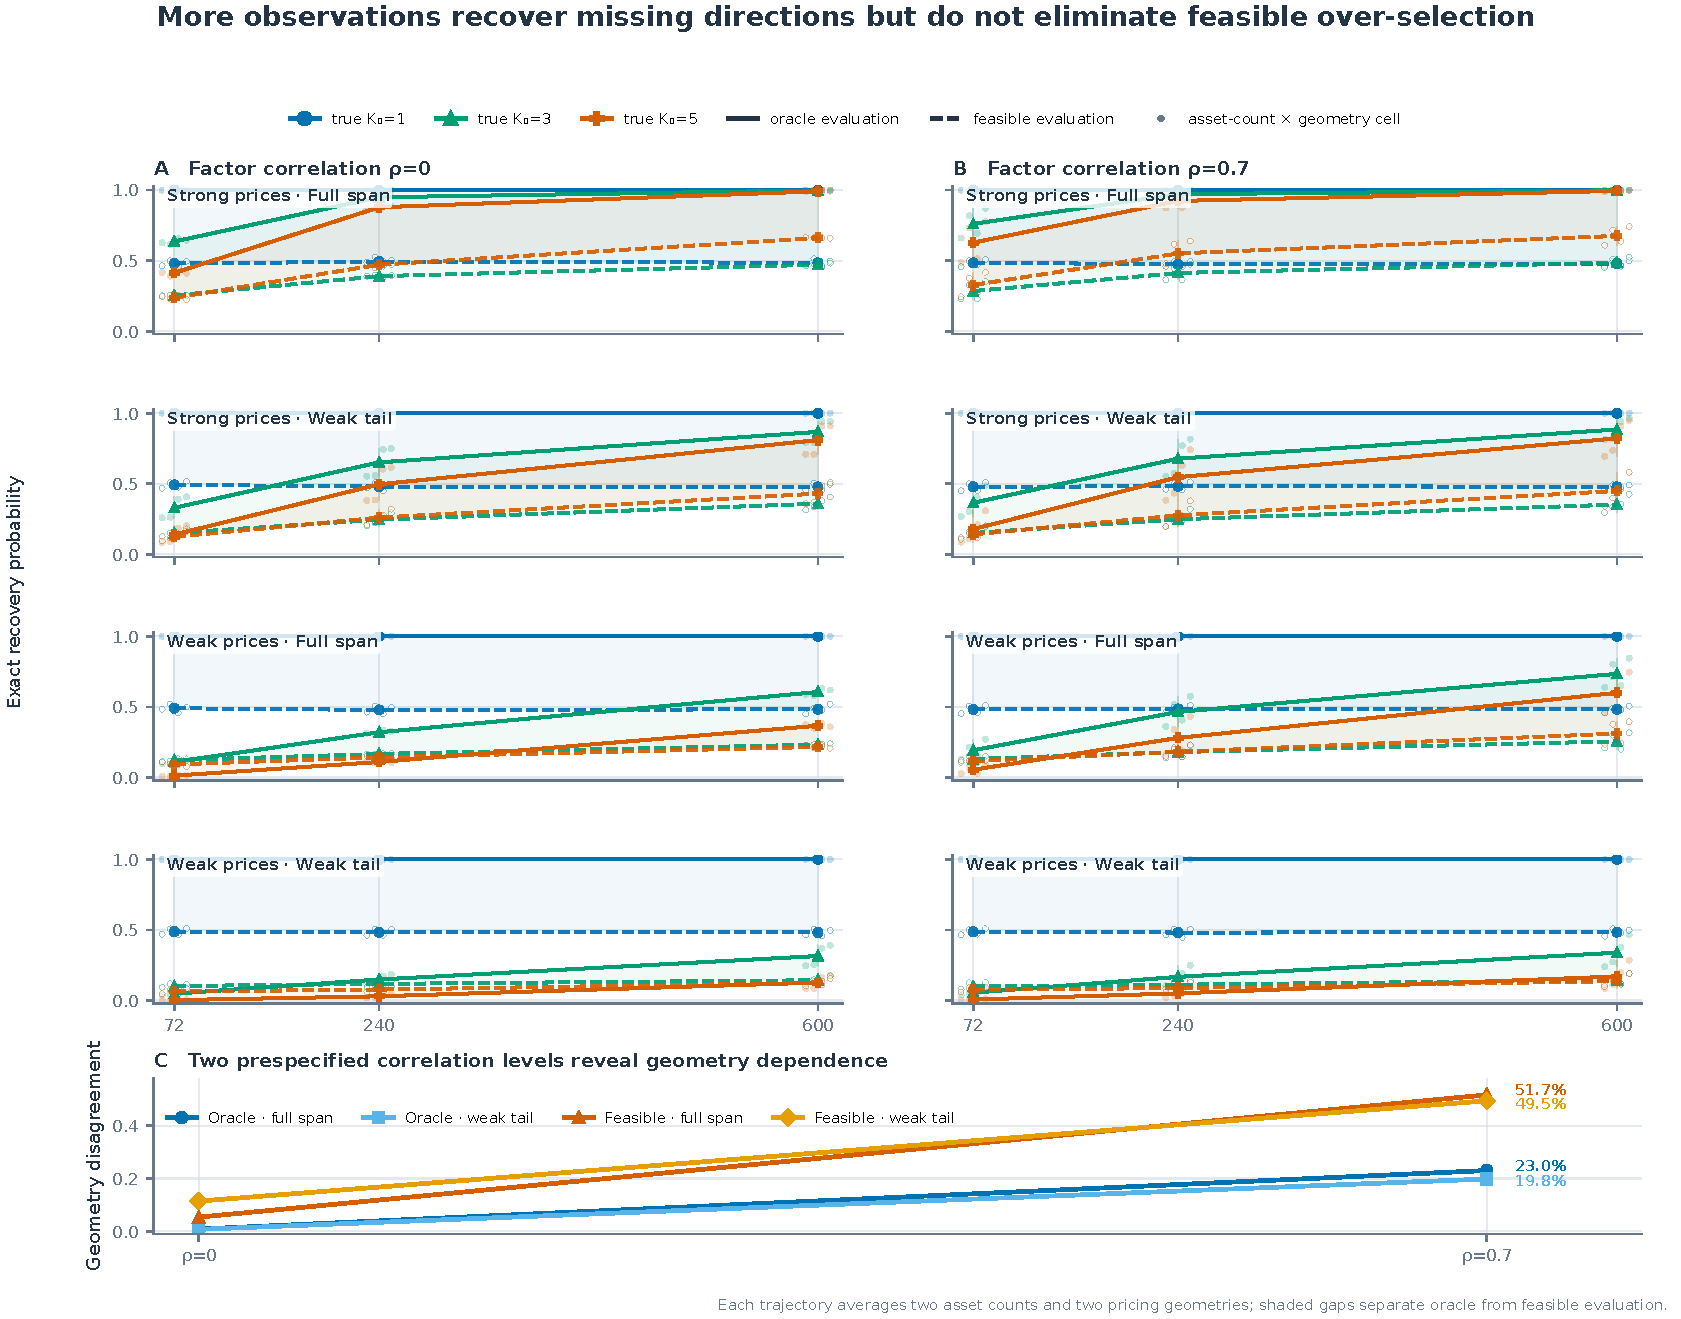
\includegraphics[width=0.99\textwidth]{figures/figure_05_identification_mechanisms.pdf}
\caption{Known-truth identification trajectories over the complete frozen condition grid. Panels A and B plot exact recovery at the three prespecified sample lengths, 72, 240, and 600 months, under factor correlations zero and 0.7. Rows distinguish risk-price strength and asset spanning; colors identify $K_0$; solid and dashed lines separate oracle and feasible evaluation. Small points expose the four asset-count--pricing-geometry cells behind each mean marker; their vertical range is also shown. Each mean is therefore based on 12,000 selection outcomes. Shaded gaps show the loss from feasible evaluation. Panel C is a two-level slope graph, rather than an interpolated correlation curve, and reports equal-versus-HJ dimension disagreement at the two prespecified correlation values.}
\label{fig:identification-dashboard}
\end{widefigure}

The result illustrates Proposition~\ref{prop:inconsistency}. Models above $K_0$ add directions with zero population price. Their empirical losses fluctuate around the same population value, so the strict minimum rewards whichever redundant direction happens to reduce sample loss. More data shrink all differences, but they do not force the sign of a centered, second-order difference to favor the minimal model. In the aggregate feasible design, the over-selection rate is 33.5\%; it rises from 31.3\% at 72 months to 35.7\% at 600 months rather than disappearing.

\subsection{Asset spanning and geometry disagreement}

Weak-tail spanning reduces the loadings on the final true directions to 0.15 of their baseline magnitude. Exact recovery falls by 12.0 percentage points, and the probability that six asset families select different dimensions rises by 7.4 points. Under oracle evaluation, multiple dimensions appear across the six families in 27.8\% of strong/full conditions, 55.1\% of strong/weak-tail conditions, and about 63--65\% of weak-price conditions. Under feasible evaluation, cross-family diversity appears in 98--99\% of conditions. A common economic dimension can therefore generate heterogeneous empirical dimensions when assets reveal its weaker directions unevenly.

Equal and HJ geometries disagree on the selected dimension in 20.3\% of all simulation cases. With independent factor directions and full spanning, disagreement is only 0.8\% under oracle evaluation and 5.3\% under feasible evaluation. Raising factor correlation to 0.7 increases those rates to 23.0\% and 51.7\%. Panel C of Figure~\ref{fig:identification-dashboard} displays this amplification.

The simulation does not identify which mechanism causes each empirical result. It establishes that the specified combinations of weak prices, weak spanning, correlated risks, weighting, and evaluation noise can generate unstable selection. The design contrasts do not imply that each mechanism alone explains the empirical results. It would be invalid to invert the simulation and declare the true empirical dimension or the causal share of each mechanism.

\subsection{Acceptable dimension sets}

The empirical object should reflect the identification result. Let $\widehat \Loss(K)$ be a validation loss and let $c_T(K)$ measure its uncertainty relative to the minimum. We define an acceptable set
\begin{equation}
 \widehat{\mathcal A}_{\delta}=\left\{K:\widehat\Loss(K)-\min_j\widehat\Loss(j)\leq c_T(K)+\delta\right\},
\end{equation}
where $\delta$ is an economically chosen tolerance. A proposed parsimonious summary is the smallest member of $\widehat{\mathcal A}_{\delta}$, accompanied by the full set, results under multiple $W$ matrices, and seed dispersion. This rule makes the identifying assumption visible. It also matches the decision problem: if several dimensions price the target assets within estimation and economic tolerance, the data support predictive equivalence, not a uniquely measured structural count.

This set is a proposed reporting device, not a confidence set validated in this study. Coverage depends on how the simultaneous uncertainty term is constructed; pointwise intervals alone do not establish it.

\section{Temporal instability and economic usability}

This section provides supporting evidence for the real-time-use stage of the framework. Because it studies independent stock-return predictors rather than the 30 pricing-dimension networks, it does not by itself show that the latent pricing dimension changes through time. Direct evidence on the dimension comes from the Core-86 development and locked pricing tests in Section~4. The forecast replay uses future-validation eligibility and complete-state-history screens, historical preprocessing, and previously selected neural hyperparameters. It is consequently a retrospective selected-sample comparison, not a fully prospective investable backtest; lagged policy decisions alone do not remove these sample and design qualifications.

\subsection{Does routine updating improve forecasts?}

The preceding analysis shows that the selected pricing dimension changes across its two nonoverlapping Core-86 periods. A natural response is to update the model frequently. The separate return-prediction replay evaluates updating, without testing a policy for choosing pricing dimension. Across 239 months and 1,043,511 stock-month observations, the frozen neural model has mean monthly squared loss 0.034313. The rolling 60-month model has loss 0.034451, and the expanding-history model has loss 0.034762. Relative to a zero forecast, their $R^2$ values are 0.261\%, $-0.140$\%, and $-1.042$\%. The point estimates favor the frozen model, although the inference does not establish that updating is universally harmful.

The full-sample average hides temporal heterogeneity. Equation~\eqref{eq:update-decomp} separates the magnitude of each model change from whether that change points toward subsequently realized returns. The two loss columns in Table~\ref{tab:temporal-economic} report the resulting update-minus-frozen differences for all three learners. For the neural model, the underlying components explain the change of sign. For rolling updates in 2000--2009, adjustment cost $A=0.000583$ dominates alignment benefit $2B=0.000051$, so updating raises loss by 0.000531. In 2010--2019, adjustment is smaller and alignment rises to 0.000509, producing a loss improvement of 0.000252. The ex-post optimal shrinkage intensity $\lambda^*=\operatorname{clip}(B/A,0,1)$ moves from 0.044 to 0.991. Expanding neural updates do not show the same reversal: their alignment remains too weak in both decades.

\begin{widetable}[!tbp]
\centering
\begin{minipage}{\textwidth}
\caption{Forecast updating and portfolio performance by learner and update rule}
\label{tab:temporal-economic}
\footnotesize
\setlength{\tabcolsep}{4pt}
\renewcommand{\arraystretch}{1.16}
\begin{tabular*}{\linewidth}{@{\extracolsep{\fill}}llrrrrrr@{}}
\toprule
 &  & \multicolumn{2}{c}{Updated minus frozen loss} & \multicolumn{4}{c}{Value-weighted portfolios; 25 bp cost} \\
\cmidrule(lr){3-4}\cmidrule(l){5-8}
Learner & Rule & 2000--09 & 2010--19 & Return (\%) & Sharpe & Turnover & CE (\%) \\
\midrule
Neural & Frozen & 0.000 & 0.000 & 13.02 & 0.546 & 1.219 & -1.20 \\
 & Rolling 60 & 0.531 & -0.252 & -0.61 & -0.022 & 0.874 & -20.32 \\
 & Expanding & 0.806 & 0.094 & 13.12 & 0.444 & 1.352 & -8.68 \\
\addlinespace[5pt]
Ridge & Frozen & 0.000 & 0.000 & 5.59 & 0.245 & 0.787 & -7.47 \\
 & Rolling 60 & 2.040 & 0.013 & 4.60 & 0.158 & 1.030 & -16.63 \\
 & Expanding & 0.031 & -0.331 & 7.92 & 0.378 & 0.745 & -3.04 \\
\addlinespace[5pt]
Tree & Frozen & 0.000 & 0.000 & 3.83 & 0.120 & 1.030 & -21.55 \\
 & Rolling 60 & 1.122 & -0.873 & -11.65 & -0.371 & 1.324 & -36.23 \\
 & Expanding & -0.771 & -1.650 & -0.16 & -0.005 & 1.148 & -22.38 \\
\bottomrule
\end{tabular*}
\par\vspace{4pt}
{\footnotesize\raggedright\textit{Notes:} Loss differences are multiplied by $10^3$; negative values favor updating. Zero for the frozen rule is the comparison baseline. Portfolio return and certainty equivalent (CE, risk aversion five) are annualized percentages over February 2000--December 2019. Turnover is monthly for unit long and unit short positions after return drift. Portfolio columns cover the full period, not the individual decades in the loss columns. These are separate return-prediction learners, not the pricing-dimension networks. None of the six update-minus-frozen return differences passes the Holm-adjusted 5\% gate.\par}
\end{minipage}
\end{widetable}


The identity has an economic interpretation. A model can adapt strongly and still fail because its changes are orthogonal to, or negatively aligned with, subsequent errors. Conversely, a modest change can add value if it consistently corrects the frozen error. ``Parameter drift'' is therefore insufficient. The direction of the drift relative to future pricing mistakes is what matters.

\subsection{Cross-estimator evidence and memory length}

Ridge and shallow tree models help separate a neural-network peculiarity from a broader updating tradeoff. For rolling 60-month estimates, both the neural and tree models move from adjustment-cost dominance in the 2000s to alignment-benefit dominance in the 2010s. The tree update changes from a loss increase of 0.001122 to a loss reduction of 0.000873. Ridge rolling updates improve substantially but remain slightly costly in the second decade.

Long-memory results are estimator-specific. Expanding Ridge improves the frozen forecast in the 2010s, and the expanding tree improves it in both decades; expanding neural updates do not. No update window is universally optimal. What travels across model classes is a higher alignment of model changes with subsequent frozen-model errors in the later sample, especially for short-memory fits. The economic tradeoff is between responsiveness to drift and estimation variance, and that tradeoff depends on the learner.

High realized stock-market variance raises losses for all three neural policies. The high-variance state is the only one of four frozen environment definitions that remains significant for all policies after Holm adjustment and across HAC bandwidths. This result does not prove a change in the conditional-mean mapping, because the squared-error target mechanically contains more return noise in volatile months. It is reported as performance heterogeneity, not structural attribution.

\subsection{Retrospective change versus real-time detection}

Using the full 2000--2019 sample, the six standardized model--window advantage series share an estimated break after April 2014. The exploratory joint block-bootstrap $p$-value is 0.0214, and all six mean changes are positive. The bootstrap interval for the first post-break month runs from October 2009 to January 2015, however, which is wide relative to a real-time trading horizon.

The historical CUSUM exercise is more demanding. Its threshold of 5.6178 is calibrated on 2000--2009 to target a nominal 5\% probability of one or more false triggers over 120 months under the bootstrap calibration distribution. The statistic does not cross that threshold until August 2018; updating begins in September and is active for only 16 of the 120 evaluation months. The neural switch improves on the frozen model by only 0.000048 per month, with a confidence interval containing zero and Holm $p=1.000$. It underperforms always rolling by 0.000204, with Holm $p=0.0405$. Ridge and tree switch rules also fail their prespecified advancement comparisons.

This gap between 2014 and 2018 is central. A change can be detectable after accumulating the complete post-break record and still be too weak or gradual to identify promptly under false-alarm control. Lowering the threshold after observing the delay would use future information and turn a failed test into specification search. The frozen rule is therefore closed rather than tuned.

\subsection{Portfolio implementation}

The portfolio columns in Table~\ref{tab:temporal-economic} evaluate the same learner--rule combinations over the full period under the primary value-weighted, 25-basis-point specification. These columns test economic usefulness separately from the decade-specific forecast losses. The frozen neural strategy has the largest Sharpe ratio, 0.546, and annualized net return of 13.02\%. Rolling neural updating reduces the return to $-0.61$\% and raises no economic-use claim. Expanding neural updating has a similar return to the frozen policy but a lower Sharpe ratio. Ridge expanding performs better than frozen Ridge in point estimates, while both tree updates are weaker than frozen tree.

None of the six update-minus-frozen return differences survives the prespecified Holm 5\% gate. The neural rolling policy trails frozen by 1.136 percentage points per month; its unadjusted $p=0.0122$ becomes Holm $p=0.0732$. The positive Ridge-expanding difference has an interval containing zero and Holm $p=1$. Every value-weighted strategy has a negative certainty equivalent at risk aversion five.

Costs materially affect ranking. The frozen neural annualized return falls from 16.68\% with zero cost to 9.36\% at 50 basis points. Ridge expanding falls from 10.15\% to 5.68\%, and tree expanding from 3.29\% to $-3.60$\%. The result is consistent with the broader point that model comparison can change after turnover is priced \citep{detzel2023costs}. Predictive updating and economic updating are distinct endpoints.

Figure~\ref{fig:temporal-dashboard} links the three temporal hurdles: forecast adjustment can reverse sign across decades, the real-time rule detects the retrospective break with a long delay, and every primary after-cost certainty equivalent remains negative.

\begin{widefigure}[!tbp]
\centering
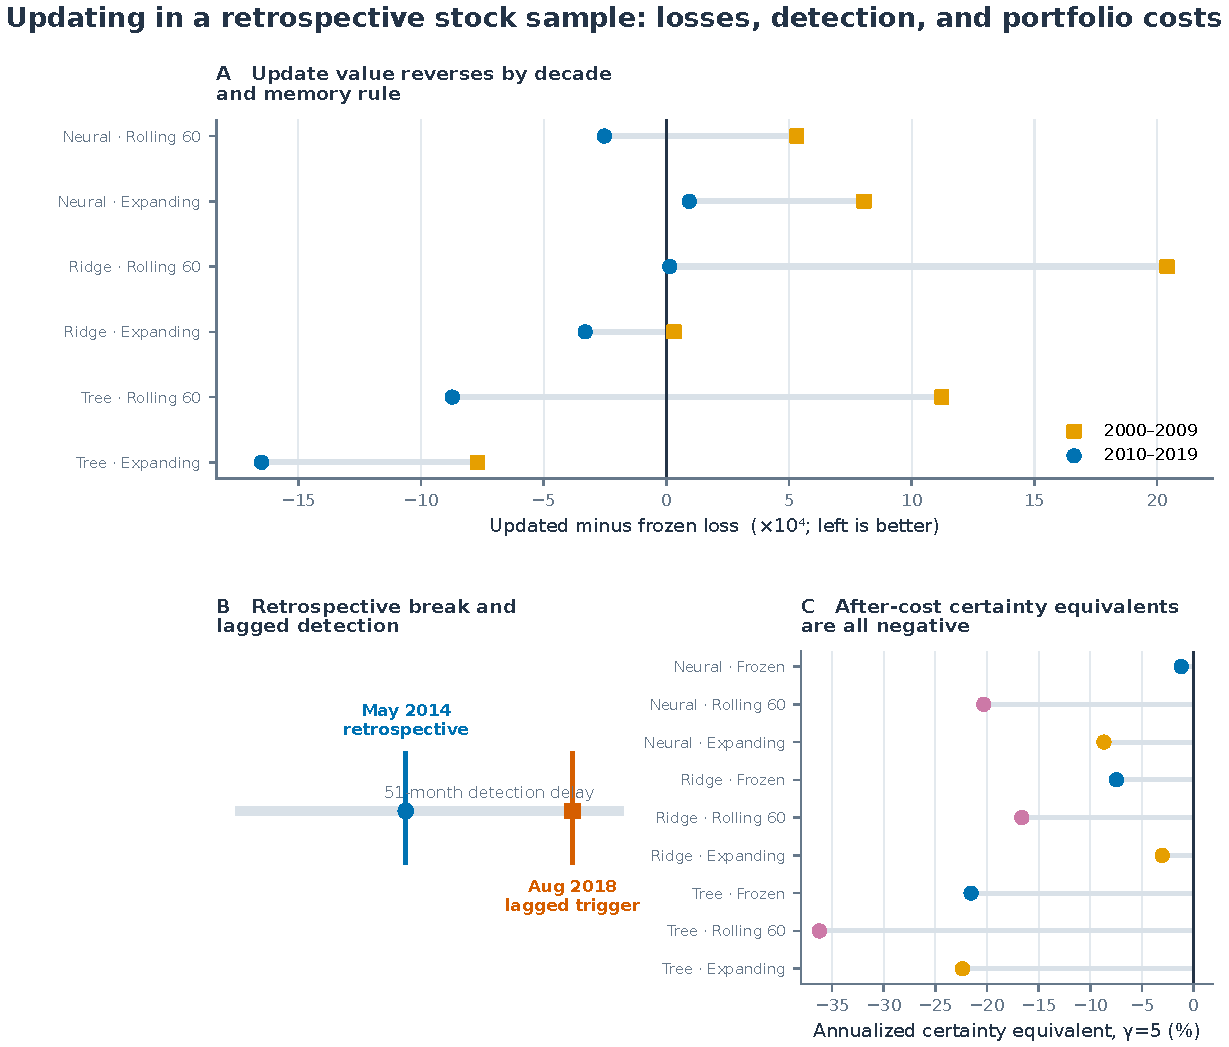
\includegraphics[width=0.99\textwidth]{figures/figure_06_temporal_usability.pdf}
\caption{Temporal usability dashboard. Panel A reports updated-minus-frozen loss by learner, memory rule, and decade. Panel B contrasts the exploratory retrospective break with the frozen real-time CUSUM crossing. Panel C reports annualized certainty equivalents for the value-weighted 25-basis-point primary portfolios.}
\label{fig:temporal-dashboard}
\end{widefigure}

\subsection{Implication for temporal dimension claims}

Temporal instability does not imply that a researcher should continually change $K$ or retrain every parameter. A low-dimensional representation can remain geometrically compact while the risk prices attached to its directions, its asset exposures, or the usefulness of its forecast changes evolve. The current evidence locates a change in update alignment, but it does not yet separate exposure-span rotation from risk-price migration in the full 30-model family. That attribution is outside the evidence reported here.

For the evidence available here, the appropriate conclusion is narrower. Updating value varies over time and can be visible retrospectively. The tested lagged detector does not identify that change early enough to establish incremental value in this internal replay. Therefore a time-varying pattern cannot be used as evidence for a stable, real-time economic state variable unless the detection and implementation gates pass separately.

\section{What does the network geometry establish?}

\subsection{Layerwise concentration across normalization rules}

Hidden representations become more concentrated with depth under all three normalization rules (Table~\ref{tab:geometry}). Each row describes one layer under one normalization; the columns distinguish spectral concentration, local dimension, tangent-angle diagnostics, and temporal drift. Under raw centering, median participation rank falls from 20.251 in hidden layer 1 to 14.669 in layer 2 and 9.048 in layer 3. Feature z-scoring produces 22.989, 16.538, and 10.476; row-$L_2$ normalization produces 21.168, 15.479, and 9.105. The decline is therefore not driven by a single coordinate scale.

\begin{widetable}[!tbp]
\centering
\begin{minipage}{\textwidth}
\caption{Layerwise representation geometry under three normalization rules}
\label{tab:geometry}
\footnotesize
\setlength{\tabcolsep}{4pt}
\renewcommand{\arraystretch}{1.16}
\begin{tabular*}{\linewidth}{@{\extracolsep{\fill}}lrrrrrrr@{}}
\toprule
Layer & Participation & Entropy & PCA95 & TWO-NN & LB ($k=20$) & Tangent angle & Drift \\
 & rank & rank & rank & dimension & dimension & (radians) & (rank 5) \\
\midrule
\multicolumn{8}{@{}l}{\textit{A. Raw centering}} \\[2pt]
Hidden 1 & 20.251 & 35.855 & 50 & 15.477 & 13.835 & 1.493 & 0.987 \\
Hidden 2 & 14.669 & 23.760 & 32 & 14.072 & 12.054 & 1.474 & 0.862 \\
Hidden 3 & 9.048 & 13.839 & 18 & 11.814 & 9.757 & 1.437 & 0.670 \\
\addlinespace[5pt]
\multicolumn{8}{@{}l}{\textit{B. Feature z-score}} \\[2pt]
Hidden 1 & 22.989 & 38.444 & 51 & 15.750 & 14.186 & 1.494 & 0.942 \\
Hidden 2 & 16.538 & 25.430 & 32 & 14.237 & 12.399 & 1.477 & 0.890 \\
Hidden 3 & 10.476 & 15.097 & 18 & 11.990 & 10.058 & 1.429 & 0.661 \\
\addlinespace[5pt]
\multicolumn{8}{@{}l}{\textit{C. Row-$L_2$ normalization}} \\[2pt]
Hidden 1 & 21.168 & 36.728 & 50 & -- & -- & -- & 0.948 \\
Hidden 2 & 15.479 & 24.609 & 32 & -- & -- & -- & 0.856 \\
Hidden 3 & 9.105 & 13.903 & 18 & -- & -- & -- & 0.661 \\
\bottomrule
\end{tabular*}
\par\vspace{4pt}
{\footnotesize\raggedright\textit{Notes:} Entries are archived medians for 30 frozen networks and 120 development months. Spectral summaries use 3,600 observations per group; drift uses 3,570 adjacent-month pairs. Neighbor dimensions and tangent angles use only 300 observations per raw/z-score group (ten sampled months). LB is the Levina--Bickel estimator. Dashes denote diagnostics not computed under row normalization, not zero values. The numerical-collapse rate is zero; it is not a classification neural-collapse test. The two adjacent-layer CKA medians are 0.875 and 0.848. These are descriptive, finite-scale diagnostics; the separate economic-function test is reported in Figure~\ref{fig:evidence-ladder} and Section~6.3.\par}
\end{minipage}
\end{widetable}


Independent synthetic calibration precedes the empirical estimates. The first calibration failed two of six gates because a fixed tangent-space rank could not distinguish curved from flat manifolds and the scale-artifact design did not match the z-score estimand. Those failures were retained. A corrected, frozen calibration chose local rank adaptively and aligned the scale design with the estimand; it passed plane dimensions 3 and 8, curvature, collapse, scale-artifact, and full-rank anisotropy gates. This supports use of the estimators as directional diagnostics, not as an oracle for unique intrinsic dimension.

The collapse rate is zero. The final layer's leading-eigenvalue share is 0.232 and its PCA90 and PCA95 dimensions are 14 and 18. Hence the pattern is anisotropic concentration rather than a representation converging to a constant or a one-dimensional line. Z-scoring increases final-layer participation rank by 1.427, or 15.8\%, which confirms some scale influence but remains far below the frozen 50\% artifact threshold.

\subsection{Concentration is not evidence of a smooth pricing manifold}

The term ``manifold'' suggests more than a low effective rank. It suggests that observations lie near a smooth lower-dimensional object whose local tangent spaces vary coherently. The finite-scale tangent-angle diagnostic is insufficient to establish that interpretation. Its median declines from 1.493 to 1.437 radians rather than increasing with depth. Values near a right angle indicate that local and larger-scale tangent estimates are not tightly aligned. The representation is concentrated, but the evidence does not establish a unique smooth manifold.

Adjacent-layer CKA medians are 0.875 for hidden 1 versus hidden 2 and 0.848 for hidden 2 versus hidden 3. Layers retain much of the same cross-sectional structure while reorganizing it. Rank-five monthly Grassmann drift falls from 0.987 to 0.862 and 0.670 across layers. Deeper principal subspaces are more stable over adjacent months even though they are not fixed.

High-volatility months have a final-layer raw participation rank only 0.165 above other months. The small association does not identify a volatility-driven state transition. It also illustrates why a geometrically stable subspace and a stable pricing function are different claims: the subspace can move less while the output weights or realized price of risk change materially.

\subsection{The prespecified economic-function gate fails}

The descriptive compression does not pass the separate economic-function criterion. Figure~\ref{fig:evidence-ladder} displays the model-level prediction errors. The primary probe predicts each model's development-period HJ loss from final-layer geometry after controlling for nominal factor count. Validation leaves out one seed at a time so that a seed-specific geometry--performance relation cannot be evaluated on the same seed used to fit it. Adding geometry reduces RMSE from 0.106 to 0.102, an improvement of 3.915\%. This is below the prespecified 5\% threshold, and the within-factor-count permutation $p$-value is 0.149. The within-factor-count Pearson correlation is $-0.296$.

The secondary factor-Sharpe endpoint has permutation $p=0.041$ but improves RMSE by only 1.211\%. It cannot replace the failed HJ endpoint. Searching another layer, normalization, state split, or economic outcome after seeing the result would convert a prespecified test into an unbounded geometry search. The analysis therefore stops at the planned gate.

\begin{widefigure}[!tbp]
\centering
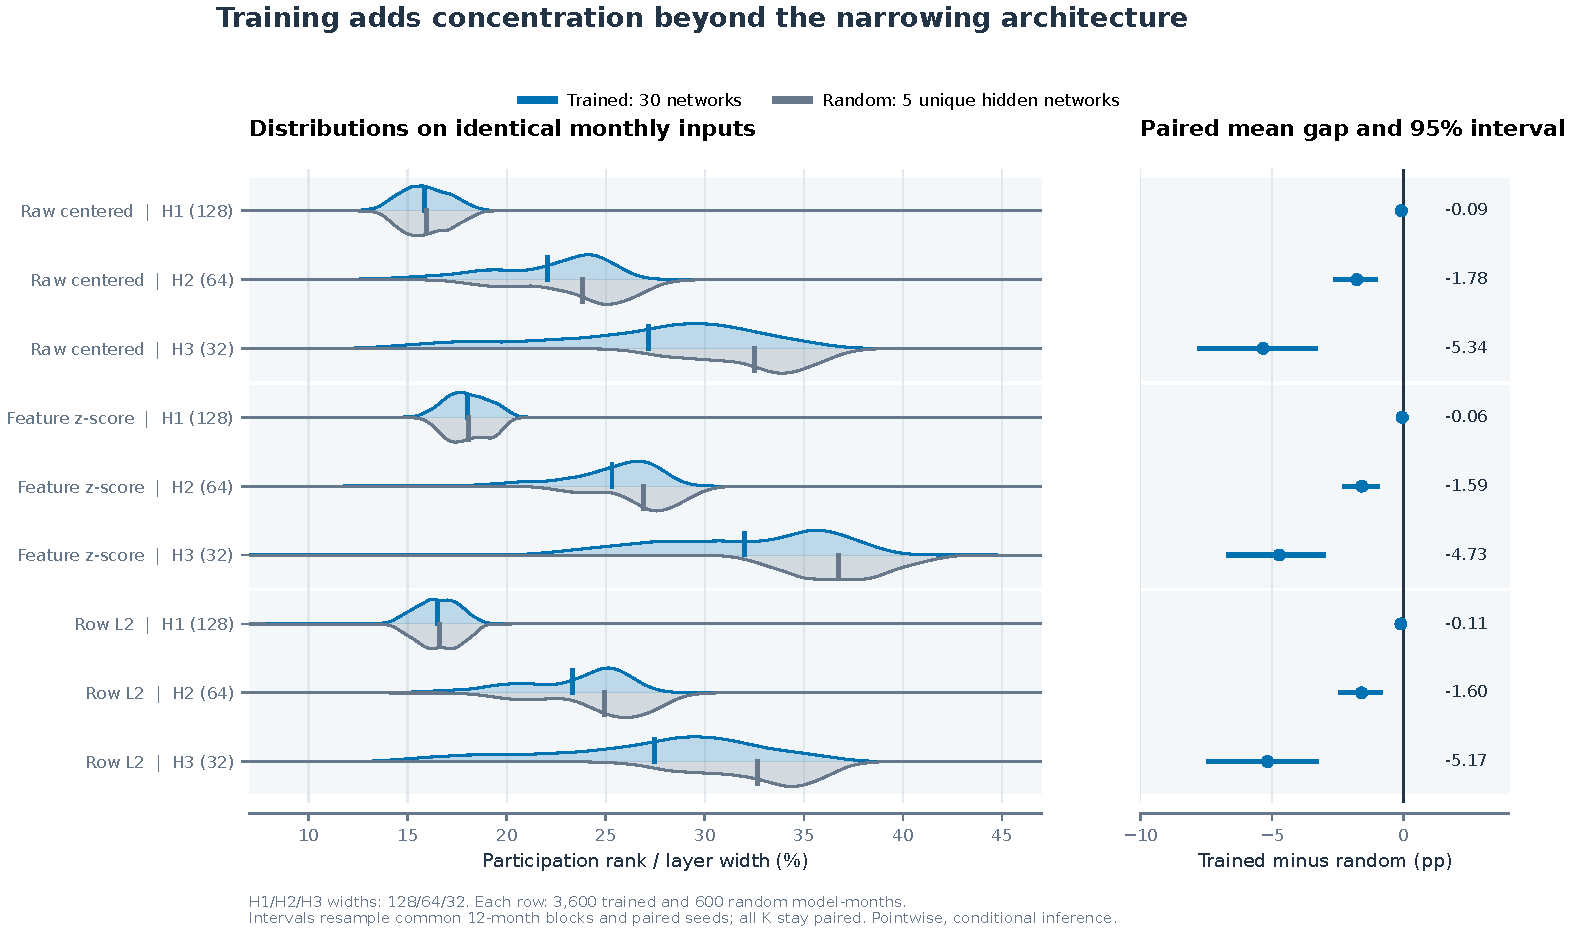
\includegraphics[width=0.98\textwidth]{figures/figure_07_geometry_function.pdf}
\caption{Distribution of layerwise concentration across all 32,400 frozen model--month--layer--normalization cells. Each ridge contains 3,600 observations. Filled distributions pool months; solid orange and dashed gray contours separate high-volatility and other months. Diamonds mark participation-rank medians and are colored by median rank-five month-to-month Grassmann drift. Within each normalization, arrows connect the three layer medians. Compression and declining drift are pervasive rather than artifacts of a few model averages, while the annotated functional probe remains below its prespecified 5\% HJ-loss gate.}
\label{fig:geometry-dashboard}
\end{widefigure}

The result clarifies what high-dimensional networks may be doing. They organize 86 characteristics and 86 missingness indicators into progressively concentrated internal coordinates, and those coordinates become somewhat more stable with depth. But concentration does not reveal the number of priced shocks. It may reflect denoising, redundancy removal, saturation, common firm-characteristic structure, or an architecture-induced spectral bias. For the proposed incremental pricing interpretation, the geometry must predict pricing moments, SDF performance, or exposure spans beyond what nominal factor count already explains. The prespecified probe does not provide that incremental evidence here.

\subsection{Connecting geometric and economic compression}

The empirical pieces are consistent without being identical. The hidden representation concentrates to an effective rank near nine, while endpoint pricing choices range among one, two, four, five, and eight depending on data and loss. There is no contradiction: effective rank counts active variation in hidden activations, whereas pricing dimension counts directions needed to reduce a particular set of Euler errors. Some active hidden directions can support nonlinear sorting without carrying distinct risk prices. Some weak priced directions can have little activation variance and still matter under an HJ geometry or for a targeted asset family.

The economic direction of compression provides the bridge. Development decompositions show that a dominant common payoff direction explains part of the geometry contrast. The hidden-state evidence shows a broad anisotropic representation rather than a literal one-factor code. One interpretation is that a few common directions contain much of the variation, while additional directions may refine relative pricing. These diagnostics do not identify that hierarchy within individual hidden units. Which refinement counts as necessary depends on asset spanning, the metric, measurement, and the historical risk-price configuration.

This hierarchy is more informative than a single bottleneck number. It suggests reporting a spectrum, an acceptable dimension set, and economic labels for identifiable directions. The common market direction may be more stable than the exact position at which validation loss reaches its minimum. That is the sense in which compression can be economically interpretable without being a stable law of exact dimension.

\section{Discussion and conclusion}

\subsection{Interpretation of the evidence}

Within the tested model family, hidden activations concentrate across layers, but the preferred pricing dimension depends on the assets, weighting, seed, archived data pipeline, and period. These observations concern different objects. Effective rank measures the distribution of activation variance. Pricing loss measures errors for a specified payoff span. Selecting a small output width under one loss therefore does not establish that the hidden representation has that dimension, or that the economy contains that number of priced shocks.

The market-direction diagnostics offer a limited economic interpretation. Removing a validation-estimated market component reduces the geometry contrast in the later period in point estimates, while adding the market factor does not jointly improve raw moments and alphas. This is consistent with a distinction between dominant common variation and relative-pricing errors. The wide attenuation intervals and pipeline sensitivity prevent a precise attribution of compression losses to market risk. We do not estimate the causal contributions of state complexity, risk exposures, and risk prices.

The known-loading example explains why larger samples need not make the raw validation minimum select the smallest correct span. Redundant directions can exploit evaluation-mean noise even when the population mean is already spanned. It does not establish that this mechanism accounts for all empirical switches. Non-nested fitted networks, optimization error, regularization, and measurement changes can also alter rankings.

\subsection{Reporting and practical implications}

A dimension claim is easier to assess when researchers report all candidate losses, algorithmic dispersion, and a stated tolerance for practically equivalent performance. A penalized or tolerance-based selector needs its own justification and validation. The acceptable-set formulation in Section~4 is a reporting proposal; the present study does not estimate its coverage or demonstrate that it outperforms existing selection procedures.

Asset choice and weighting should accompany the reported dimension. Equal-moment loss, regression alpha, and a regularized HJ-type norm emphasize different features of pricing errors. Data provenance is equally relevant. The Core-92/Core-86 contrast shows sensitivity between two archived pipelines, but does not isolate the information content of six deleted characteristics. Exact source vintages, timing conventions, and missingness treatment are needed to interpret such a comparison.

For model monitoring, retrospective deterioration is a reason to investigate a specification, not evidence that immediate retraining will improve it. The update-loss identity separates the size of a forecast change from its alignment with subsequent errors. In the tested replay, favorable later-period alignment did not translate into a successful real-time switching criterion or a statistically significant primary incremental portfolio gain. This evidence concerns the specified learners, detector, costs, and sample; it does not rule out useful updating policies elsewhere.

\subsection{Limitations}

The empirical pricing family is a diagnostic family that did not pass earlier benchmark-advancement criteria. It is not a representative sample of all successful machine-learning asset-pricing models. The results concern U.S. equities and conventional numerical characteristics; other markets, payoff spans, objectives, and architectures may behave differently.

Chronology limits the strength of the confirmation claim. Core-86 used a target-month cutoff before 2020 and fixed models for the later evaluation, but legacy development had already included January 2020. Moreover, the temporal switching design followed inspection of the broader development history. Its lag-respecting replay is internal evidence, not independent prospective validation. The temporal panel also conditions on future-validation eligibility and complete state histories, and uses historically selected preprocessing and neural hyperparameters. Its trading results cannot be interpreted as a fully ex-ante investable-universe backtest. These limitations are disclosed rather than repaired by relabeling observed periods as fresh holdouts.

The characteristic bridge uses benchmark values where available and reconstructed values otherwise. It is not an independent point-in-time reconstruction of the historical information set. Current-vintage accounting revisions, coverage differences, and the legacy timing shift can contribute to measured instability. Licensed raw records cannot be included in the public package; aggregate exhibit replay and full reconstruction with licensed source vintages are separate reproducibility tasks.

Geometry is measured at a finite cross-sectional sample and neighborhood scale. A tangent-angle diagnostic is not an estimate of a unique smooth pricing manifold, and zero numerical collapse does not test the supervised neural-collapse phenomenon studied in classification. The functional probe has 30 models and five seed folds, so a failed threshold does not prove zero economic information in every geometric statistic. The study also leaves causal attribution to state, exposure, and risk-price changes unresolved.

\subsection{Conclusion}

Low-dimensional descriptions and economic dimension claims require different evidence. Our pricing networks exhibit concentrated activations, while their preferred output dimensions change across evaluation designs. A known-loading simulation demonstrates persistent over-selection from noisy validation, and the separate updating exercise finds no significant primary incremental after-cost gain under the tested rule. The resulting conclusion is conditional: report compactness as a property of the fitted representation, and report pricing dimension with its asset span, loss, uncertainty, data construction, and chronology. These diagnostics delimit the structural interpretation supported by the present evidence.


\section*{Data availability}
The replication package provides construction and analysis code, frozen configurations, synthetic results, aggregate figure and table data, and checksums. The package follows the section order of this article. CRSP, Compustat, CCM, and third-party security-level characteristic records, model checkpoints, stock-level predictions, and derived security-level panels are excluded. Their inputs and reconstruction paths are documented for researchers with the required access. Public source downloads are linked rather than relicensed. Reproducing the published exhibits from aggregate outputs is distinct from rerunning the full licensed-data pipeline.
\ifdefined\IRFAAUTHORED
The versioned replication package is archived at \url{https://doi.org/10.5281/zenodo.23064062}. Its development repository is \url{https://github.com/extradimen/asset-pricing-dimension-replication}. Version 1.0.0 accompanies this manuscript.

The archive should be cited as \citet{wang2026replication}.
\else
Repository identifiers are provided in the separate title-page file for editorial access.
\fi

\ifdefined\IRFAAUTHORED
\section*{Funding}
This research received no specific grant from any funding agency in the public, commercial, or not-for-profit sectors.

\section*{Declaration of competing interest}
The authors declare that they have no known competing financial interests or personal relationships that could have appeared to influence the work reported in this paper.

\section*{CRediT authorship contribution statement}
\textbf{Jinpeng Wang:} Conceptualization, Methodology, Software, Data curation, Formal analysis, Visualization, Writing -- original draft, Writing -- review \& editing.
\textbf{Yan Jiang:} Supervision, Validation, Writing -- original draft, Writing -- review \& editing.

\fi

\section*{Declaration of generative AI and AI-assisted technologies in the manuscript preparation process}
During the preparation of this work, the authors used OpenAI Codex to assist with literature organization, code development and auditing, artifact indexing, statistical-figure production, and language drafting. The authors reviewed and edited all generated material, verified cited sources and numerical claims against frozen project evidence, and take full responsibility for the content of the article.

\begingroup
\small
\setlength{\bibsep}{3pt}
\urlstyle{same}
\bibliographystyle{elsarticle-harv}
\bibliography{references/references}
\endgroup
\end{document}
